\documentclass[a4paper,12pt]{article}
\usepackage[utf8]{inputenc}
\usepackage{amsmath}
\usepackage{amsfonts}
\usepackage{amssymb}
\usepackage{graphicx}
\usepackage{caption}
\usepackage{subcaption}
\usepackage{float}
\usepackage{siunitx}
\usepackage{booktabs}
\usepackage{hyperref}
\usepackage{titling}

\title{Analisi Circuiti Derivatore e Intergatore}
\author{Francesco Giuseppe Minisini}
\date{\today}

\begin{document}
\maketitle
\hrule
\vspace{9pt}
\begin{abstract}
    Nelle seguenti esperienze di laboratorio sono stati realizzati su "breadboard" circuiti di tipologia Derivatore RC e Integratore RC. Ne si è studiato il comportamento nel dominio del tempo e rilevandone, tramite oscilloscopio, l'andamento del segnale di tensione in uscita $v_{out}(t)$ sottoposti a diversi segnali in ingresso $v_{in}(t)$ di frequenze e forme d'onda variabili, in modo da confrontare le misure ottenute con i risultati previsti dall'analisi teorica e da simulazioni eseguite tramite "LTspice". Si è inoltre studiato il comportamento nel dominio della frequenza di circuiti Derivatoere RC e Integratore RC mediante il tracciamento dei diagrammi di Bode per guadagno in decibel $G(f)$ e sfasamento $\phi(f)$, confrontando le misure sperimentali con i risultati delle simulazioni.
\vspace{20 pt}
\hrule
\end{abstract}
\vspace{2 pt}


% \hrule
% \maketitle
% \vspace{9pt}
% \begin{abstract}

    %     \noindent
%     Nell'esperienza sono replicati i circuiti derivatore, integratore e trigger di schmidt. La procedura sperimentale consiste in una fase di preparazione del layout di ciascun circuito e, dopo esserci accertati della correttezza di essi, la connessione di essi alle componenti di alimentazione e di generazione di segnali. Una volta reso operativo il circuito, abbiamo eseguito la misura di diverse grandezze. 
%     Per il circuito Integratore e Derivatore abbiamo ricostruito il diagramma di Bode in decadi, misurando Guadagno e Fase nel dominio della frequenza.  
%     per il trigger di schmidt abbiamo misurato la soglia di scatto a data frequenza, e studiato il ciclo di steresi ottenuto attraverso il diagramma di Nyquist.
%     I risultati ottenuti sono risultati interessanti, e talvorta inaspettati, ma si nota piena corrispondenza con i risultati delle simulazioni.
% \vspace{20 pt}
% \hrule
% \end{abstract}
% \vspace{2 pt}

% % \begin{figure}[H]
% %     \centering
% %     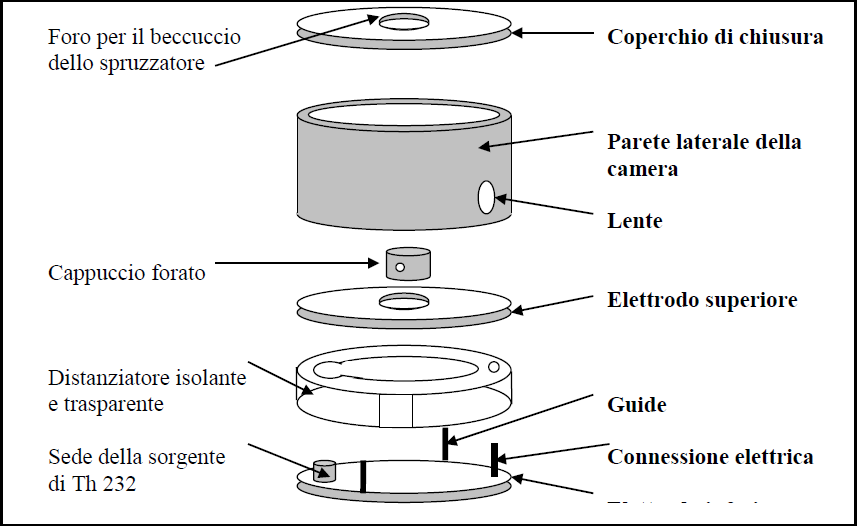
\includegraphics[width=0.6\textwidth]{Apparato2.png}
% %     \caption{Schema dell'apparato sperimentale completo.}
% %     \label{fig:apparato_completo}
% % \end{figure}


% % \begin{figure}[H]
% %     \centering
% %     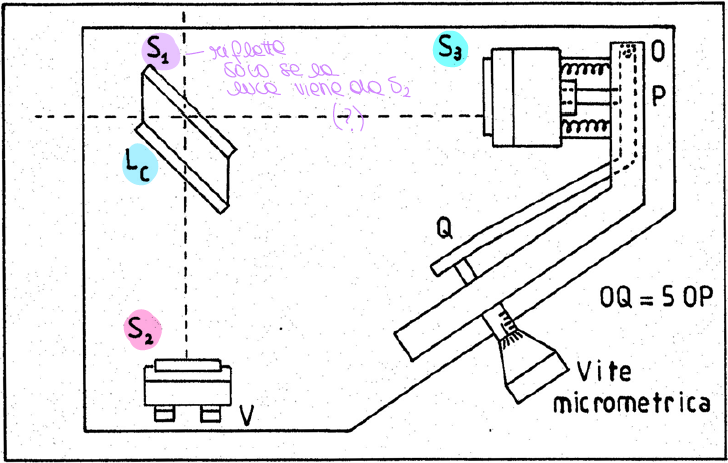
\includegraphics[width=0.7\textwidth]{apparato1.png}
% %     \caption{Sistema di lenti dell'apparato sperimentale.}
% %     \label{fig:Sistema_lenti}
% % \end{figure}



% \section{Circuito Derivatore}
% \subsection{Assemblaggio del circuito}
% Come prima cosa abbiamo seleizionato i componenti necessari, Successivamnete abbiamo iniziato ad assemblare il circuito sulla breadbord. Per prima cosa abbiamo posizionato il l'amplificatore operazionale \(LM741\) a cavallo tra le due regioni separate della breadbord con la pallina segnata rivolta verso l'alto.
% Successivamente abbiamo collegato il condensatore \(C_1\) dalla capacità elettrica di \(C_1 = 46.8nF\) alla porta d'ingresso numero \(2\) rendendo così il circuito di tipo invertente.
% Dopo averlo correttamente posizinato abbiamo collegeto la resistenza \(R_1 = 2.2k\Omega \) all'uscita dell'amplificatore operazionale numer 6 e alla porta di ingresso dell'amplificatore numero 2.
% Successivamente abbiamo collegato il terminale positivo della porta "Output" del generatore di onde sinosuidali al componente \(C_1\) e quello negativo a terra. 
% Preparato il circuito abbiamo assemblato l'alimentazione dell'amplificatore operazionale, collegando il generatore di tensione all'amplificatore operazionale, in modo tale da fornire tensione costante di \(V_3 = -12V \) alla porta di ingresso 4 e di \(V_2 = 12V\) alla porta 7 di uscita.
% Per ottenere questa alimentazione abbiamo utilizzato due uscite diverse del generatore di tenzione, nel caso di \(V_3\) abbiamo collegato a terra il terminale negativo, mentre con \(V_2\) quello positivo. 
% Successivamente aìci siamo assicurati che tutte le terre nel circuito fossero constistenti, collegando perciò i terminali positivi di V2 e negativi di V3 alla terra del genaratore di onde sinosuidali.
% Completa l'assemblaggio del circuito abbiamo preparato l'oscilloscopio, come prima cosa abbiamo collegato all'uscita output il  canale 1 o \(CH1\), oltere al circuito l'oscilloscopio attraverso uno sdoppiatore, e la sonda, collegata all uscita "output" ossia la 4 dell'amplificatore.
% Dopo aver collegato anche i generatori ed esserci assicurati della correttezza del circuito, in particolare della orienzazione dell'amplificatre, che metterebbe a rischi il componente, abbiamo attivato prima l'alimentazione dell'amplificatore e successivametne il generatore di onde sinosuidali, impostato ad una ampiezza fissa di \(Amplitude_{V_1} = 200m\). 
% Abbiamo percò ottenuto un circuito derivatore operativo.

% \vspace{0.5cm} % Aggiungi un po' di spazio dopo l'abstract
% \begin{abstract}

\section{Richiami teorici}
Dal punto di vista teorico, i circuiti derivatore RC, integratore RC e il trigger di Schmitt possono essere analizzati utilizzando la legge dei nodi di Kirchhoff (KCL, ``Kirchhoff's Current Law''), secondo cui la somma delle correnti entranti in un nodo è uguale alla somma delle correnti uscenti. Questo approccio consente di ottenere equazioni differenziali che descrivono il comportamento della tensione in uscita \( v_{out}(t)\) (o semplicemente \(v_{out}\)), definita come la tensione misurata ai capi del circuito in uscita, rilevata in laboratorio tramite un oscilloscopio collegato a un’opportuna sonda.

\subsection{Circuito Derivatore RC}
Il circuito derivatore RC è composto da un condensatore di capacità \( C \) in serie con l’ingresso e un resistore di resistenza \( R \) collegato a terra, come illustrato dall'immagine \ref{fig: derivatore}. La tensione in ingresso \( v_{in}(t) \) è il segnale applicato al circuito, mentre \( v_{out}(t) \) è la tensione in uscita. Applicando la KCL al nodo tra il condensatore e il resistore, e considerando il principio della terra virtuale (tensione al nodo di uscita dell’amplificatore operazionale pari a zero), si ottiene:
\begin{equation}
    i_C(t) = i_R(t)
\end{equation}
Dove \( i_C(t) \) è la corrente attraverso il condensatore e \( i_R(t) \) è la corrente attraverso il resistore. Esplicitando le correnti in termini di differenze di potenziale:
\begin{equation}
    C \frac{d(v_{in}(t) - 0)}{dt} = \frac{0 - v_{out}(t)}{R}
\end{equation}
Risolvendo rispetto a \( v_{out}(t) \):
\begin{equation}
    \label{derivatore}
    v_{out}(t) = -RC \frac{d v_{in}(t)}{dt} = -\tau \frac{d v_{in}(t)}{dt}
\end{equation}
Dove \( \tau = RC \) è la costante di tempo del circuito, con \( R \) espressa in ohm (\( \Omega \)) e \( C \) in farad (\( F \)). L’uscita è proporzionale alla derivata temporale della tensione in ingresso.

Se il segnale in ingresso è sinusoidale, \( v_{in}(t) = V_A \sin(2\pi f_0 t) \), dove \( V_A \) è l’ampiezza del segnale (in volt) e \( f_0 \) è la frequenza del segnale (in hertz), l’uscita diventa:
\begin{equation}
    \label{sin_derivatore}
    v_{out}(t) = -2\pi f_0 RC V_A \cos(2\pi f_0 t) = 2\pi f_0 RC V_A \sin\left(2\pi f_0 t + \frac{3\pi}{2}\right)
\end{equation}
L’ampiezza dell’uscita è proporzionale a \( 2\pi f_0 RC \), indicando che il guadagno aumenta linearmente con la frequenza. Nel dominio della frequenza, il diagramma di Bode del modulo presenta una pendenza costante di \( +20 \, \text{dB/decade} \).

\subsection{Circuito Integratore RC}
Il circuito integratore RC è composto da un resistore di resistenza \( R \) in serie con l’ingresso e un condensatore di capacità \( C \) collegato tra l’uscita e il nodo virtuale a terra, assemblati come riportato nella figura \ref{fig: integratore}. Anche qui, \( v_{in}(t) \) è la tensione in ingresso e \( v_{out}(t) \) è la tensione in uscita. Applicando la KCL al nodo di terra virtuale:
\begin{equation}
    \frac{v_{in}(t)}{R} = -C \frac{d v_{out}(t)}{dt}
\end{equation}
Risolvendo rispetto a \( v_{out}(t) \):
\begin{equation}
    v_{out}(t) = -\frac{1}{RC} \int_0^t v_{in}(t') \, dt' + v(0)
\end{equation}
Dove \( v(0) \) è la condizione iniziale della tensione sul condensatore al tempo \( t = 0 \), e \( \tau = RC \) è la costante di tempo. L’uscita è proporzionale all’integrale della tensione in ingresso.

Per un ingresso sinusoidale \( v_{in}(t) = V_A \sin(2\pi f_0 t) \), con \( V_A \) e \( f_0 \) definiti come sopra, l’uscita è:
\begin{equation}
    \label{eq: integratore_sin}
    v_{out}(t) = \frac{V_A}{2\pi f_0 RC} \cos(2\pi f_0 t) + v(0) = \frac{V_A}{2\pi f_0 RC} \sin\left(2\pi f_0 t + \frac{\pi}{2}\right) + v(0)
\end{equation}
L’ampiezza dell’uscita è inversamente proporzionale a \( 2\pi f_0 RC \), indicando che il guadagno decresce con la frequenza. Il diagramma di Bode del modulo ha una pendenza costante di \( -20 \, \text{dB/decade} \).

% \subsection{Trigger di Schmitt}
% Il trigger di Schmitt è un circuito con retroazione positiva, caratterizzato da un effetto di memoria dovuto alla retroazione di una frazione della tensione di uscita \( v_{out}(t) \) all’ingresso non invertente dell’amplificatore operazionale. La retroazione è determinata da un divisore di tensione formato da due resistenze, \( R_1 \) e \( R_2 \), dove \( R_1 \) è collegata tra l’uscita e l’ingresso non invertente, e \( R_2 \) tra l’ingresso non invertente e la terra. Il fattore di retroazione è dato dal rapporto \( \frac{R_1}{R_1 + R_2} \).

% Il circuito presenta un comportamento isteretico: l’uscita \( v_{out}(t) \) commuta tra due stati stabili, definiti come:
% - \( V_{out,high} \): tensione di uscita nello stato logico alto, tipicamente pari alla tensione di alimentazione positiva dell’amplificatore operazionale (es. \( +V_{CC} \), in volt).
% - \( V_{out,low} \): tensione di uscita nello stato logico basso, tipicamente pari alla tensione di alimentazione negativa dell’amplificatore operazionale (es. \( -V_{CC} \), in volt).

% Le soglie di scatto, che determinano i valori di \( v_{in}(t) \) per cui l’uscita commuta, sono definite come:
% \begin{equation}
%     V_T^+ = \frac{R_1}{R_1 + R_2} V_{out,high}, \quad V_T^- = \frac{R_1}{R_1 + R_2} V_{out,low}
% \end{equation}
% Dove \( V_T^+ \) è la soglia superiore e \( V_T^- \) è la soglia inferiore. Ad esempio, se \( v_{out} = V_{out,high} \), l’ingresso \( v_{in}(t) \) deve superare \( V_T^+ \) per commutare a \( V_{out,low} \); successivamente, \( v_{in}(t) \) deve scendere sotto \( V_T^- \) per tornare a \( V_{out,high} \). Questo comportamento può essere visualizzato tramite un diagramma di isteresi, ottenuto impostando l’oscilloscopio in modalità XY.

\subsection{Analisi nel Dominio della Frequenza}
Per l’analisi nel dominio della frequenza dei circuiti RC, il guadagno in decibel è definito come:
\begin{equation}
    \label{eq: Gdb}
    G_{dB}(f) = 20 \log_{10} \left| H(f) \right|
\end{equation}
Dove \( H(f) = \frac{v_{out}(f)}{v_{in}(f)} \) è la risposta in frequenza, con \( v_{out}(f) \) e \( v_{in}(f) \) che rappresentano le trasformate di Fourier delle tensioni di uscita e ingresso.
Per comprendere il comportamento dei circuiti RC nel dominio della frequenza, applichiamo la trasformata di Fourier alle equazioni differenziali ottenute in precedenza.

La frequenza caratteristica dei circuiti RC è data da:
\begin{equation}
  \label{eq: freqenza_carr}
    f_c = \frac{1}{2\pi \tau} = \frac{1}{2\pi RC}
\end{equation}
dove 
\begin{equation}
  \label{eq: tau}
  \tau = RC  
\end{equation}
constante di tempo del circuito.


\subsubsection*{Derivatore RC}
L’espressione nel dominio del tempo per il derivatore RC è:
\[
v_{out}(t) = -RC \frac{d v_{in}(t)}{dt} = -\tau \frac{d v_{in}(t)}{dt}
\]

Applicando la trasformata di Fourier, ricordando che:
\[
\mathcal{F}\left\{ \frac{d v_{in}(t)}{dt} \right\} = j 2 \pi f V_{in}(f)
\]

si ottiene:
\[
V_{out}(f) = -\tau (j 2 \pi f) V_{in}(f)
\]

Quindi la funzione di trasferimento nel dominio della frequenza è:
\[
H(f) = \frac{V_{out}(f)}{V_{in}(f)} = -\tau j 2 \pi f
\]

Il modulo del guadagno è:
\begin{equation}
  \label{eq:guadagno_der}
  |H(f)| = 2 \pi f \tau
\end{equation}

e la fase è:
\[
\angle H(f) = \arg(-j 2 \pi f \tau) = -\frac{\pi}{2} = -90^\circ
\]
Pertanto, il circuito derivatore amplifica le alte frequenze e introduce uno sfasamento costante di \(-90^\circ\).

\subsubsection*{Integratore RC}

Nel dominio del tempo, l’uscita del circuito integratore è:
\begin{equation}
  \label{eq:integratore}
  v_{out}(t) = -\frac{1}{RC} \int_0^t v_{in}(t') dt' = -\frac{1}{\tau} \int_0^t v_{in}(t') dt'
\end{equation}

Applicando la trasformata di Fourier, ricordando che:
\[
\mathcal{F}\left\{ \int_0^t v_{in}(t') dt' \right\} = \frac{V_{in}(f)}{j 2 \pi f}
\]

si ottiene:
\[
V_{out}(f) = -\frac{1}{\tau} \cdot \frac{V_{in}(f)}{j 2 \pi f}
\]

Quindi la funzione di trasferimento è:
\[
H(f) = \frac{V_{out}(f)}{V_{in}(f)} = -\frac{1}{j 2 \pi f \tau}
\]

Il modulo del guadagno è:
\[
|H(f)| = \frac{1}{2 \pi f \tau}
\]
e la fase è:
\[
\angle H(f) = \arg\left(-\frac{1}{j 2 \pi f \tau}\right) = +\frac{\pi}{2} = +90^\circ
\]

Ciò conferma che l’integratore attenua le alte frequenze (il guadagno decresce con \( f \)) e introduce uno sfasamento costante di \( +90^\circ \).

\subsubsection*{Riepilogo}

\[
\begin{array}{|c|c|c|}
\hline
\textbf{Parametro} & \textbf{Derivatore} & \textbf{Integratore} \\
\hline
|H(f)| & 2 \pi f \tau & \dfrac{1}{2 \pi f \tau} \\
\hline
\angle H(f) & -90^\circ & +90^\circ \\
\hline
\end{array}
\]

Questi risultati sono confermati anche sperimentalmente tramite il diagramma di Bode ottenuto in laboratorio, che mostra:
\begin{itemize}
    \item per il derivatore: pendenza di \( +20 \, \text{dB/decade} \)
    \item per l’integratore: pendenza di \( -20 \, \text{dB/decade} \)
\end{itemize}



\section{Valutazione delle incertezze sperimentali}
Le resistenze elettriche, le capacità e le induttanze dei resistori, dei condensatori e degli induttori utilizzati nell’assemblaggio di ciascun circuito sono state misurate mediante il "tester" da banco "LCR400" marchiato "Aim-Tti". Le incertezze relative a tali misure sono state stimate in base all’ordine di grandezza della sensibilità dello strumento, dedotta dal numero di cifre significative visualizzate sul display per ciascuna grandezza misurata, tenendo in considerazione anche l'oscillazione delle ultime cifre.
Le incertezze associate alle misure relative ai segnali $v(t)$ di tensione: ovvero la frequenza $f$ del segnale in ingresso, le ampiezze picco-picco $V_{pp,in}$ e $V_{pp,out}$ rispettivamente del segnale in ingresso e in uscita, nonché le eventuali misure di istanti di tempo $t$ sono state stimate come segue.

% L'incertezza sulla frequenza $f$ è stata assunta pari all'unità dell’ultima cifra significativa del valore riportato dall'oscilloscopio. Le incertezze sulle ampiezze di tensione $V_{pp,in}$, $V_{pp,out}$ e sui tempi $t$ sono state invece stimate valutando il valore di tensione o di tempo associato a un singolo pixel del display dell'oscilloscopio, facendo riferimento alla scala temporale e verticale impostata. Alcune misure sono state effettuate attraverso la funzionalità "Cursor" dell'oscilloscopio, le incertezze utilizzate per queste misure sono state stimate considerando l'incertezza associata ad un pixel relativa alla scala impostata.

L'incertezza sulla frequenza \( f \) è stata assunta pari al \( 0.4\% \) del valore misurato, in quanto l'oscilloscopio mostrava una fluttuazione di tale entità nei valori letti. Le incertezze sulle ampiezze di tensione \( V_{pp,in} \) e \( V_{pp,out} \) sono state fissate pari a \SI{4}{\milli\volt}, valore rappresentativo delle oscillazioni osservate nelle letture, in particolare quando le misure erano dell’ordine dei millivolt. Nel caso della misura delle tensioni constanti, come la tensione duale \(V_{CC\pm} \), usata per alimentare gli amplificatori operazionali, è stata utilizzata una incertezza dell'ultima cifra siglificativa segnata sul display, ossia di \(\sigma_{V_{CC} = 0.1 V}\). Per quanto riguarda le misure temporali \( t \), si è considerata la risoluzione del display e la scala impostata, assumendo come incertezza la dimensione corrispondente a un singolo quadrato della griglia del display. lcune misure sono state effettuate attraverso la funzionalità  \(Cursor\) dell'oscilloscopio, le incertezze utilizzate per queste misure sono state stimate considerando l'incertezza associata ad un pixel relativa alla scala impostata.

Nello svolgere i calcoli, l'incertezza $\sigma_G$ su ogni grandezza $G(X_1,X_2,...,X_N)$ dipendente dai valori di altre grandezze $X_1,X_2,..,X_N$ con incertezze $\sigma_{X_1}, \sigma_{X_2},..,\sigma_{X_N}$ sarà sempre calcolata tramite la formula generale di propagazione delle incertezze, secondo cui:
\begin{equation}
    \sigma_G = \sqrt{\left( \frac{\partial G}{\partial X_1} \sigma_{X_1} \right)^2 + \left( \frac{\partial G}{\partial X_2} \sigma_{X_2} \right)^2 + \dots + \left( \frac{\partial G}{\partial X_N} \sigma_{X_N} \right)^2}
\end{equation}


\section{Strumentazione Impiegata}
Ogni circuito studiato è stato assemblato su breadboard, utilizzando opportune resistenze, condensatori, induttori da laboratorio e fili conduttori rivestiti di gomma isolante.

I segnali di tensione applicati ai circuiti sono stati generati mediante l'impiego del generatore di segnali Agilent 33220A, che consente di impostare le principali caratteristiche dei segnali, quali frequenza, ampiezza picco-picco, offset e forma d’onda.

Le tensioni di ingresso e di uscita sono state rilevate tramite l’oscilloscopio digitale Tektronix TDS 2014B.

Il segnale di ingresso è stato applicato al circuito attraverso una coppia di cavi coassiali, che conducono il segnale sia al circuito che all’oscilloscopio. Il segnale in uscita, invece, è stato rilevato mediante una sonda di tensione, che lo conduce all’oscilloscopio tramite un cavo coassiale, il cui conduttore esterno è collegato a terra.

La sonda impiegata per captare il segnale in uscita può essere utilizzata in modalità "$\times 1$" o "$\times 10$". 
La seconda delle due modalità aggiunge una resistenza da $9\,\mathrm{M}\Omega$ nel circuito che conduce il segnale all'oscilloscopio. Tale resistenza è responsabile di un'attenuazione della tensione misurata di un fattore $10$.
La sonda è stata utilizzata in modalità "$\times 1$", assicurandosi di impostare la medesima modalità anche sull'oscilloscopio.

Inoltre, sul display del generatore di segnali utilizzato non viene riportato l'effettivo valore di ampiezza di tensione inviato al circuito, ma riporta l'ampiezza della tensione che vi sarebbe ai capi di una resistenza di $50\,\mathrm{M}\Omega$. E' necessario ovviare a tale problema impostando nel menu del generatore di segnali l'opzione "High $\mathrm{Z}$", in modo che venga riportato il valore di tensione ai capi di una impedenza ben maggiore di $50\,\mathrm{M}\Omega$, come è quella presente nei circuiti studiati.
% I valori in Tensioni e di frequenze osservate durante l'esperienza, sono state misurate attraverso l'uso dell'oscilloscopio. I valori di incertezza considerati per le frequenze sono stati determinate sperimentalemente: impostando un'segnale periodico sul generatore ad una data frequenza \(f_gen\), ne si è osservata la misura di questa sull'oscilloscopio e si notava una leggera oscillazione che corrispondeva a circa il \(\sigma_{f,\%} = 0.4\% \) rispetta al valore impostato sul generatore.
% Analoga procedura è stata impiegata per la stima della incertezza sui valori di delle tensioni, osservando una oscillazione dei valori misurati costante, di circa \(\sigma_v = 4 mV\).
% Per la misura


\section{Analisi dei Circuiti nel Dominio del Tempo}
\label{componenti}
Di seguito sono commentati i risultati ottenuti dallo studio dei comportamenti nel dominio del tempo dei circuiti \hyperref[sec:rc]{Derivatore RC}, \hyperref[sec:cr]{Integratore RC}, \hyperref[sec:rl]{Trigger di Schmitt}.
Si è assemblato un circuito Derivatore RC e Integratore RC impiegando un amplificatore operazionale LM741 alimentato da una Alimentazione Duale continua di \(V_{CC\pm} = (\,12.0\,\pm\,0.1\, )\, V\) dove \(V_{+}\) e \(V_{-}\) sono rispettivamente l'alimentazione positiva (pin \(7\)) e negativa (pin \(4\)), resistore di resistenza $R = (2.200\,\pm\,0.001) \,\mathrm{K}\Omega$ e un condensatore di capacità $C = (4.680\,\pm\,0.001) \,\mathrm{nF}$, dai cui valori è possibile calcolare la costante di tempo $\tau$ del circuito tramite l'equazione \ref{eq: tau}, la quale risulta pari a $\tau_{teo} = (102.96\,\pm 0.05\,) \,\mu\mathrm{s}$, da cui si ottiene, mediante l'equazione \ref{eq: freqenza_carr}, una stima della frequenza caratteristica del circuito, che viene stimata pari a $f_{caratt} = (1.5458\,\pm0.0008\,) \,\mathrm{KHz}$.
I segnali in ingresso e uscita sono stati acquisiti direttamente dall’oscilloscopio tramite una funzione interna di esportazione dei dati. Questo ci ha consentito di analizzare esattamente i valori visualizzati sul display, garantendo coerenza tra misure e grafici.
\subsection{Circuito Derivatore RC} \label{sec: rc} 
\begin{figure}[H]
  \centering
  \begin{subfigure}{0.45\textwidth}
    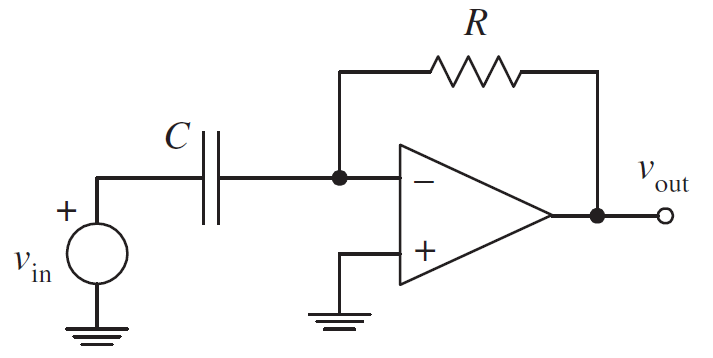
\includegraphics[width=\linewidth]{Schematic_derivatore.png}
    \caption{Schema circuitale}
  \end{subfigure}
  \hspace{0.05\textwidth}
  \begin{subfigure}{0.45\textwidth}
    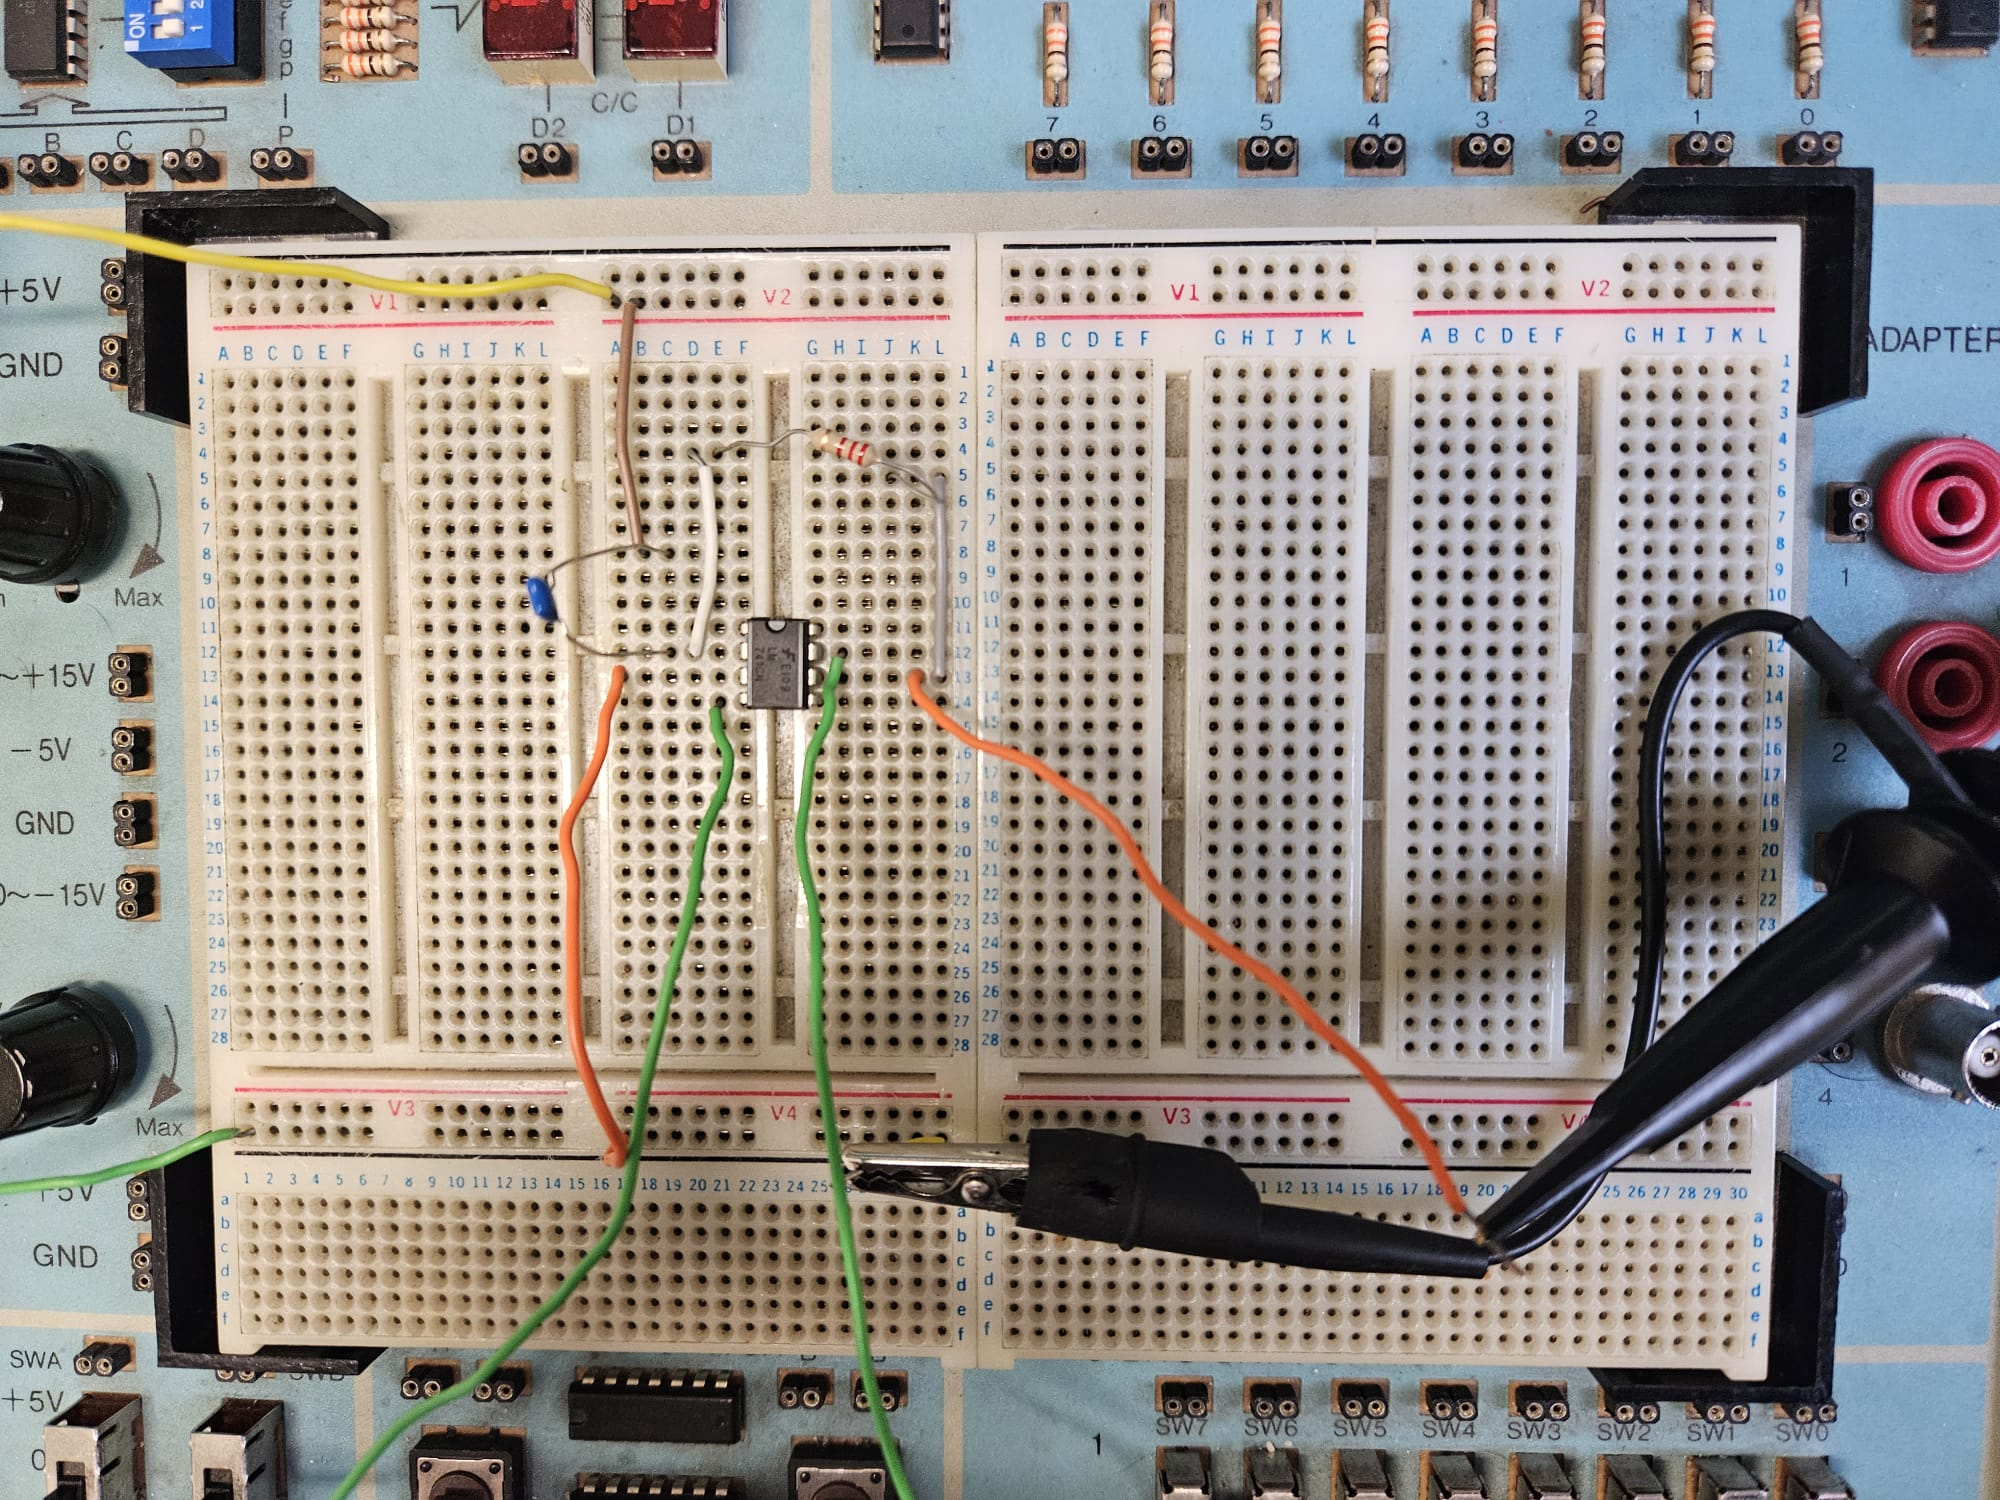
\includegraphics[width=\linewidth]{Derivatore_montato.jpg}
    \caption{Circuito assemblato}
  \end{subfigure}
  \caption{Circuito Derivatore RC}
  \label{fig: derivatore}
\end{figure}

Dopo avere assemblato il circuito Derivatore Invertente RC secondo lo schema in figura~\ref{fig: derivatore}, abbiamo testato il circuito fornendo, attraverso il generatore, segnali in ingresso \(v_{in}(t)\) di forme differenti, e osservando il comportamento della tensione in uscita \(v_{out}(t)\).

\vspace{0.3cm}
\textbf{Onda Sinosuidale.} La prima forma d'onda testata è stata un'onda sinusoidale di ampiezza \(V_{pp,in} = (202\,\pm\,4)\,\mathrm{mV}\) e frequenza \(f_{in} = (1.500\,\pm\,0.006)\,\mathrm{kHz}\), impostata tramite il generatore di funzione, sufficientemente vicino alla funzione caratteristica per ottenere un guadagno pressoché unitario, comodo per comparare le forme d'onda.

\begin{figure}[H]
  \centering
  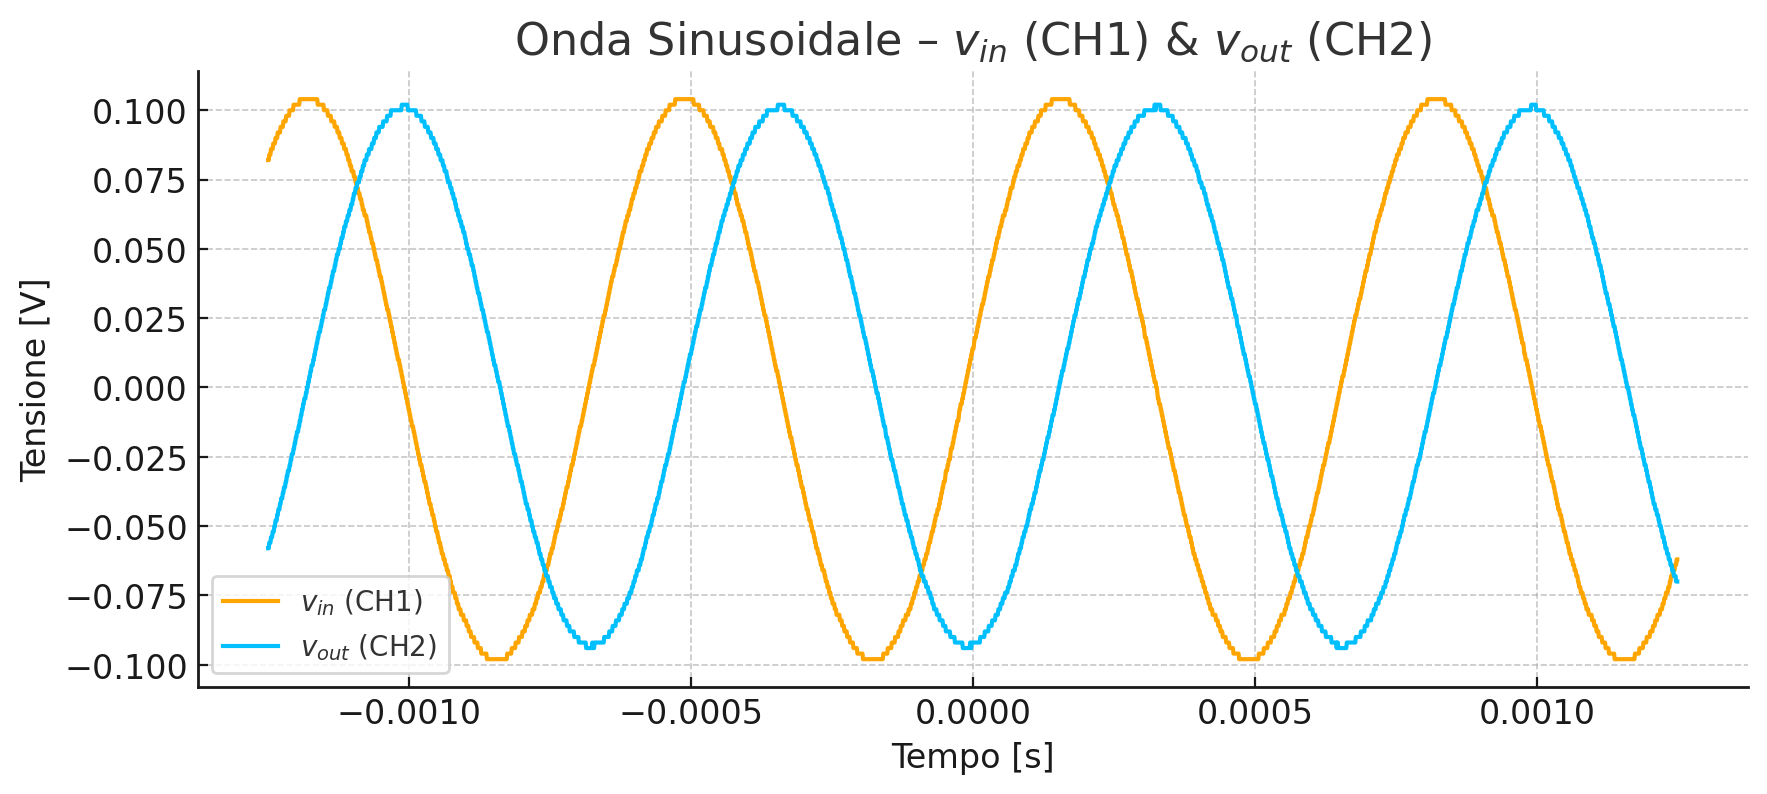
\includegraphics[width=.8\textwidth]{Sinosuidale.png}
  \caption{Derivatore RC: risposta a onda sinusoidale}
  \label{fig:derivatore_sin}
\end{figure}

Come illustrato in figura~\ref{fig:derivatore_sin}, risulta evidente che la relazione teorica \eqref{sin_derivatore} è verificata, notiamo infatti che la forma dell'onda in uscita risulta una coseno con segno meno di stessa frequenza, ma di ampiezza diversa. L'ampiezza picco-picco del segnale in uscita risulta \(V_{pp,out} = (196\,\pm\,4)\,\mathrm{mV}\), da cui otteniamo un rapporto:
\[
\left|\frac{V_{pp, out}}{V_{pp, in}}\right| = 0.97 \pm 0.03
\]

Il valore atteso per tale rapporto, secondo la relazione teorica \ref{eq:guadagno_der}, risulta:
\[
|H(f_{in})| = 0.970 \pm 0.004
\]

L'accordo è eccellente, con uno scarto relativo inferiore all'1\%. Inoltre si osserva uno sfasamento tra ingresso e uscita pari a \(\frac{3\pi}{2}\), coerente con il comportamento atteso di un derivatore invertente: l’uscita è infatti un coseno invertito.

\vspace{0.3cm}
\textbf{Onda Triangolare.} Successivamente, abbiamo testato una forma d’onda triangolare simmetrica con le stesse caratteristiche di frequenza e ampiezza. Tale forma d’onda è stata ottenuta impostando sul generatore un \textit{duty cycle} del 50\%, ottenendo un'onda triangolare perfettamente simmetrica.

\begin{figure}[H]
  \centering
  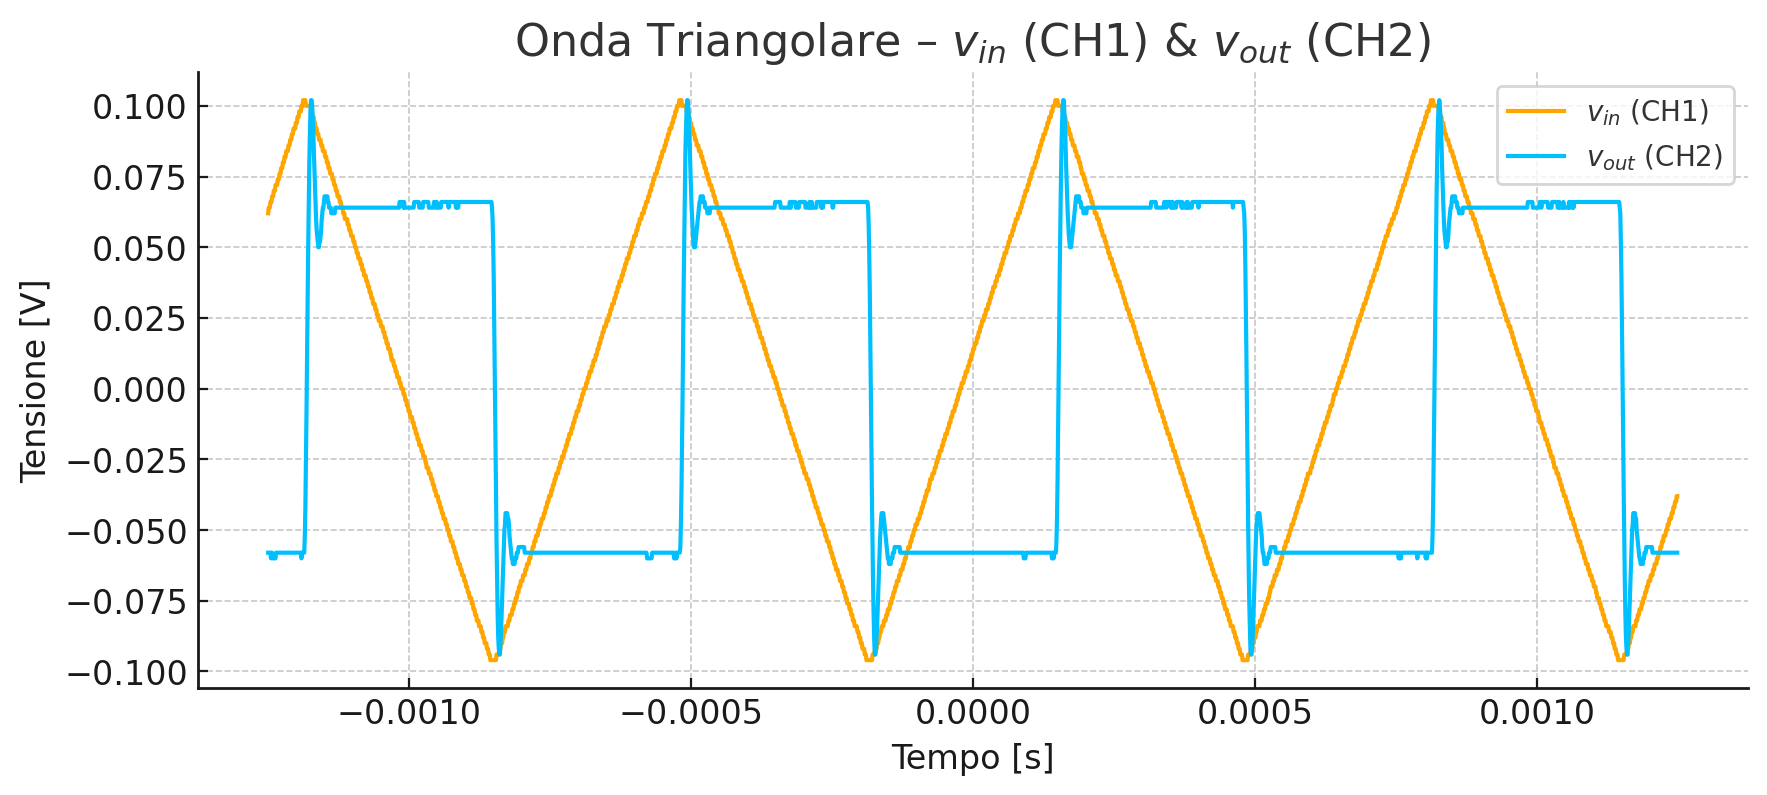
\includegraphics[width=0.8\textwidth]{Triangolare.png}
  \caption{Derivatore RC: risposta a onda triangolare simmetrica}
  \label{fig:derivatore_triang}
\end{figure}

Anche in questo caso, il comportamento osservato è in linea con le attese teoriche. La derivata di una funzione a tratti lineare, come l’onda triangolare, è una funzione costante (nei tratti lineari) con discontinuità nei punti di non derivabilità (cambio di pendenza). L’uscita risulta infatti composta da segmenti a gradino di valore costante (positivo o negativo), con rapidi transienti nei punti di inversione. L’inversione di segno del segnale in uscita rispetto alla derivata attesa conferma la natura invertente del circuito.

L’ampiezza dell’uscita nei tratti costanti risulta:
\[
V_{pp,out} = (126\,\pm\,4)\,\mathrm{mV}
\quad\Rightarrow\quad
\left|\frac{V_{out,A}}{V_{in,A}}\right| = 0.624 \pm 0.023
\]

Il valore teorico atteso, calcolando la derivata massima della triangolare come \(\left| \frac{dv_{in}}{dt} \right| = 4f V_{pp, in}\), fornisce:
\[
V_{pp,out}^{teo} = \tau 4f_{in} V_{pp, in} = 0.125 \pm 0.003\,\mathrm{V}
\]

Ancora una volta, la compatibilità è ottima, e l’accordo tra misura e teoria conferma l’accuratezza del circuito derivatore RC.

Da notare però che punti di non derivabilità, il cui segnale in uscita si traduce idealmente in un punti di discontinuità, il segnale presenta diversi picchi di ampiezza \(V_{out, peak} = (0.100\, \pm\, 0.004)\, V\), seguiti da un segnale oscillante di alta frequenza. Questo non rientra nei comportamenti attesi ed è risultato di una combinazinoi di fenomeni che allontanano il segnale da quello ideale, tra cui abbiamo il fenomento di \textit{ringing}, causato dall'induttanza e capacità parassite dei componenti. 

\vspace{0.3cm}
\textbf{Onda Quadra.}Infine, abbiamo osservato il comportamento del circuito sottoponendo l’ingresso a un’onda quadra della stessa frequenza ed ampiezza. Come previsto, l’uscita consiste in impulsi localizzati nei punti di discontinuità del segnale (i fronti di salita e discesa), mentre il segnale è pressoché nullo altrove.

\begin{figure}[H]
  \centering
  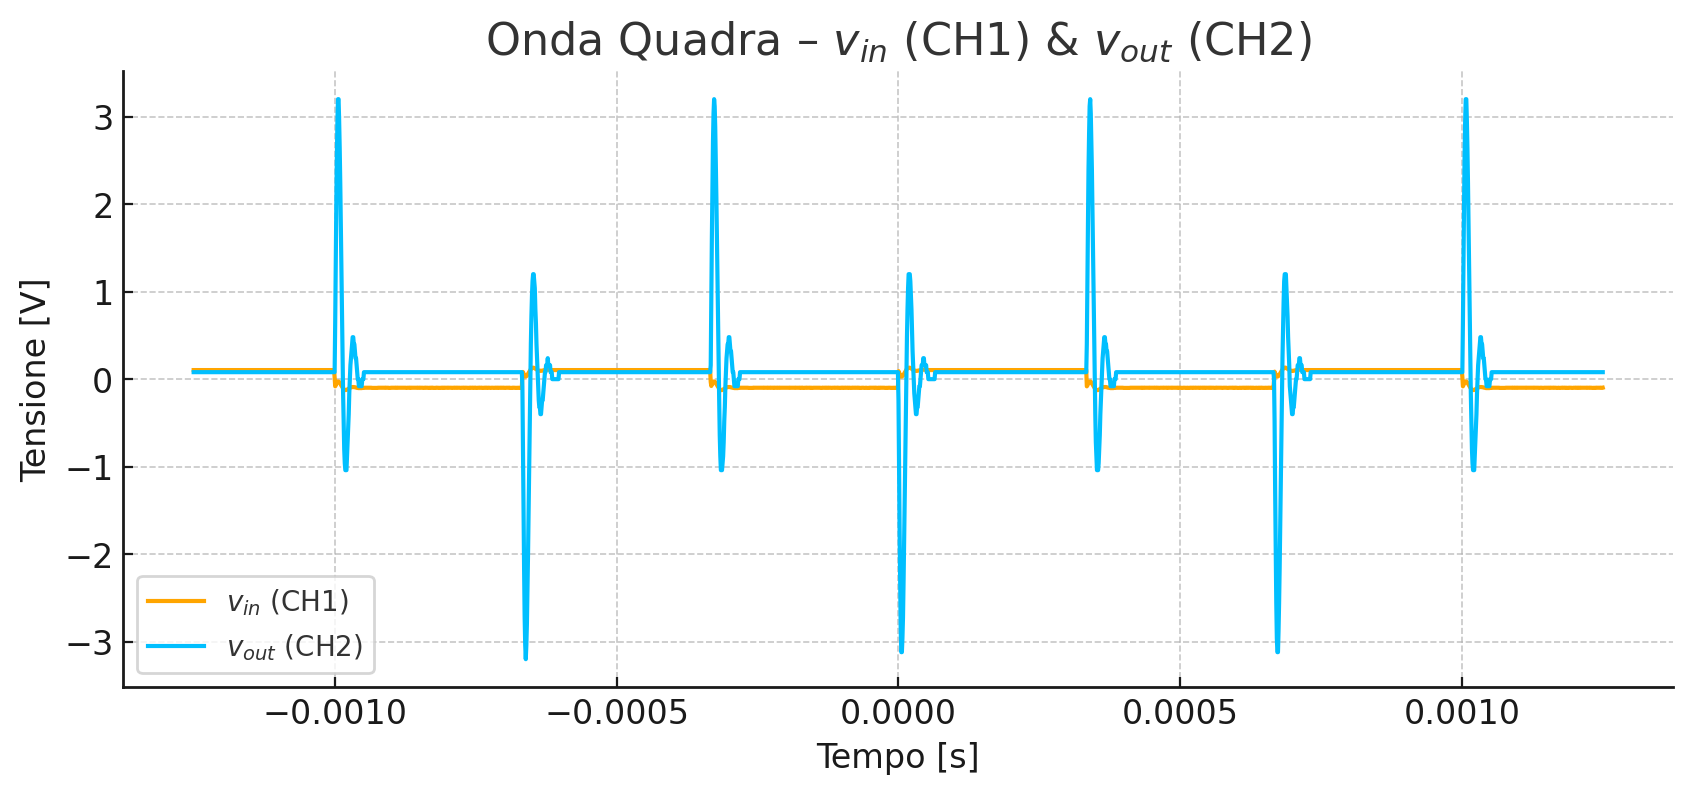
\includegraphics[width=0.8\textwidth]{Quadra.png}
  \caption{Derivatore RC: risposta a onda quadra}
  \label{fig:derivatore_quadra}
\end{figure}

L’ampiezza dei picchi misurata è \(V_{out,peak} = (3.200\,\pm\,0.004)\,\mathrm{V}\). Il valore atteso, calcolato derivando numericamente l’onda in ingresso, considerando il tempo di salita del segnale \(v_{in}\), sarebbe superiore a \(\SI{15}{\volt}\), tuttavia il limite di slew-rate dell’amplificatore LM741 (\(\approx \SI{0.5}{\volt/\micro\second}\)) introduce una saturazione dinamica, che impedisce il raggiungimento del valore teorico.
Normalmente avremmo anche anche una limitazine di tensione massima positiva \(V_{peak, +}^{max}\) e negativa \(V_{peak, -}^{max}\) che coincidono con le alimentazioni positive \(V_{CC, +}\) e negative \(V_{CC, -}\) dell'amplificatore operazionali, che quando superate il segnale viene appiattito al valore massimo. Tuttavia questo fenomeno in questo caso non rappresenta una limitazione, siccome lo \textit{slew-rate} fa in modo che, data il breve tempo di salita del segnale \(v_{in}\), il picco, la cui derivata è limitata, fa in tempo a raggiungere il valore di \(V_{out, peak}\), per poi azzerarsi quando la salita del segnale di ingresso è terminata. 
% Inoltre, l’ampiezza è limitata anche dal gain-bandwidth product dell’operazionale.

Nei punti di discontinuità si osservano inoltre delle oscillazioni (ringing) e dei transitori di durata finita. Tali anomalie sono giustificate da:

\begin{itemize}
  \item la non idealità dei componenti, in particolare induttanze parassite e capacità distribuite che creano una risposta risonante. Poichè in fatti in forme d'onda come quelle quadre sono contenute tutte le frequenze, questi effetti ne amplificano alcune, rendendole visibili;
  % \item l’effetto del tempo di salita finito del segnale in ingresso, che introduce una derivata non istantanea;
  % \item la limitata banda passante dell’amplificatore operazionale;
  \item il fenomeno di Gibbs, secondo cui la rappresentazione armonica di una discontinuità produce inevitabili overshoot.
\end{itemize}

Nonostante ciò, l’uscita mantiene il comportamento atteso di un derivatore, evidenziando chiaramente le transizioni dell’onda quadra e confermando che il circuito amplifica selettivamente le componenti ad alta frequenza.
\subsection{Circuito Integratore RC} \label{sec: int}
Abbiamo assemblato il circuito integratore RC seguendo la configurazione invertente, riportata nella figura \ref{fig: integratore} e utilizzando i componenti  elencati nella sezione \ref{componenti}. 
Anche in questo caso, abbiamo impostato una frequenza \(f_{in} = (1.500\,\pm\,0.006)\,\mathrm{kHz}\), anche in questo caso l'abbiamo impostata vicina alla frequenza caratteristica ottenendo un guadagno basso, per poter osservare con più facilità entrambe le forme d'onda ad ampiezze simili. 
L'ampiezza del segnale è stata impostata a \(V_{pp,in} = (1.50\,\pm\,0.03)\,\mathrm{V}\). L'aumento di tensione rispetto al circuito precedente ci ha permesso di visualizzare entrambe le onde sul display dell'oscilloscopio, siccome l'offset di tensione ottenuto era troppo elevato rispetto all'ampiezza del segnale per poter spostare l'onda all'interno del display.
\begin{figure}[H]
  \centering
  \begin{subfigure}{0.45\textwidth}
    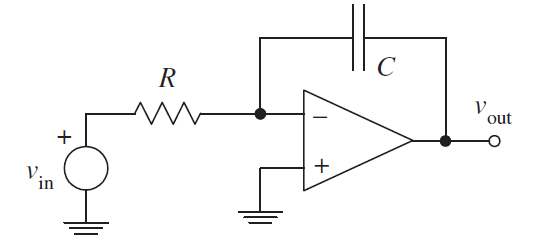
\includegraphics[width=\linewidth]{Schematic_Integratore.png}
    \caption{Schema circuitale}
  \end{subfigure}
  \hspace{0.05\textwidth}
  \begin{subfigure}{0.45\textwidth}
    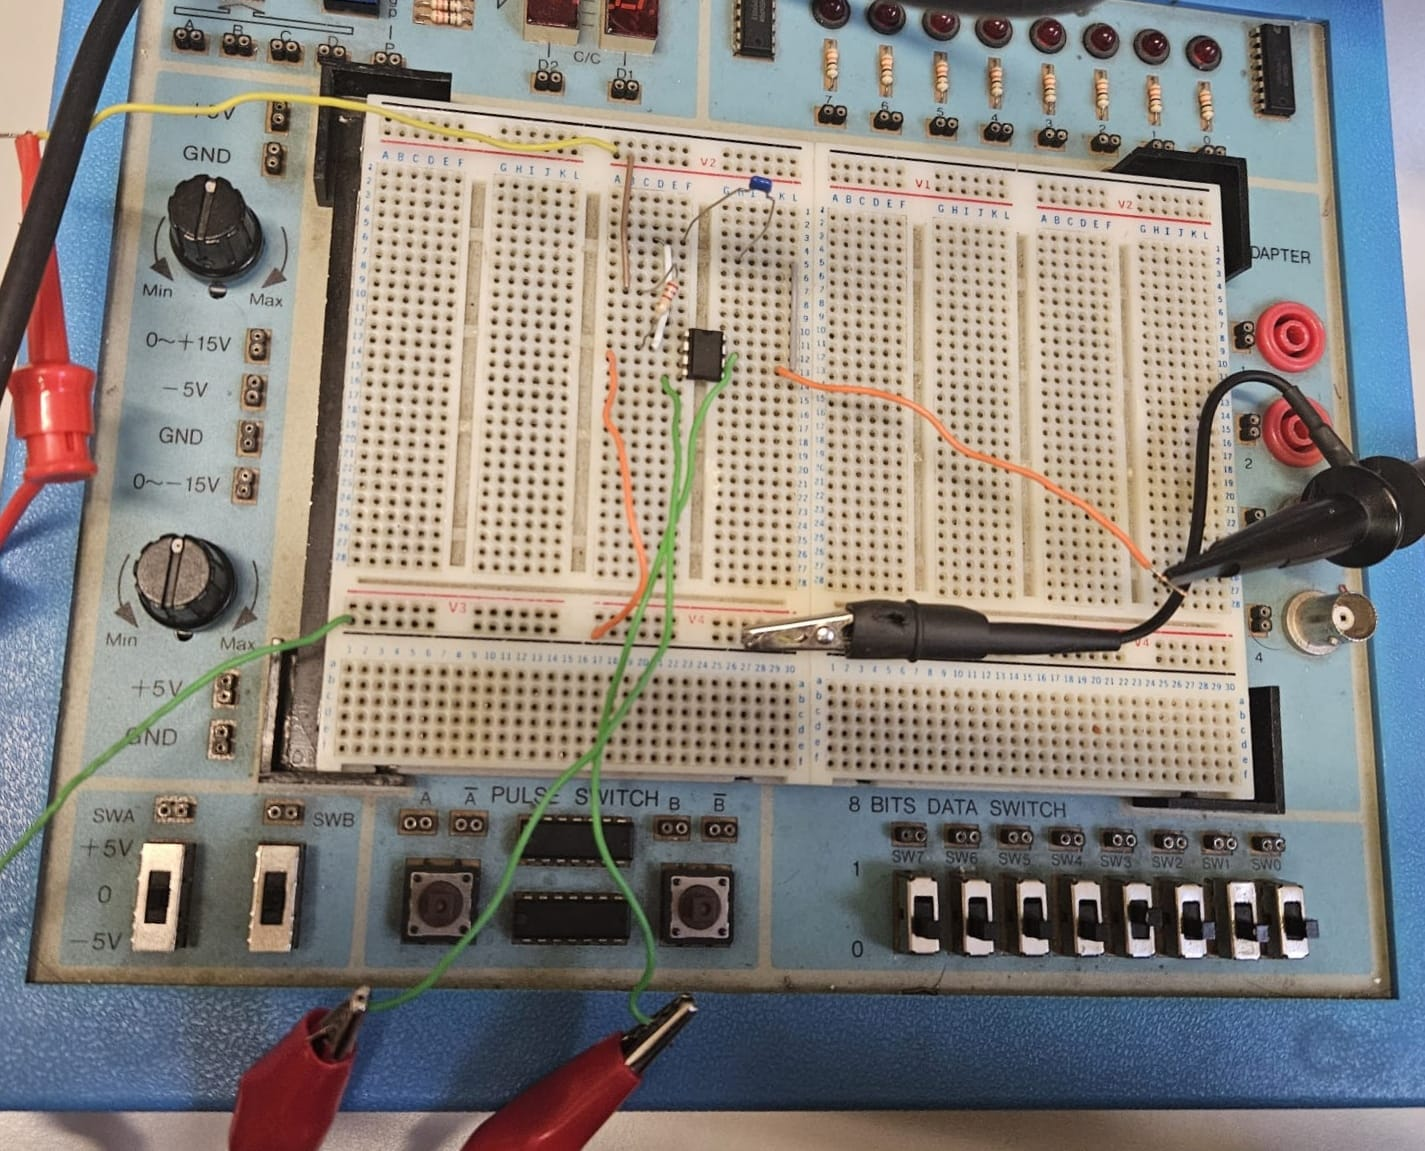
\includegraphics[width=\linewidth]{Integratore_montato.jpg}
    \caption{Circuito assemblato}
  \end{subfigure}
  \caption{Circuito Integratore RC}
  \label{fig: integratore}
\end{figure}

Durante le misure, è stata rilevata una componente di offset costante sull’uscita \(v_{out}(t)\), che è stata rimossa tramite operazione di ricentramento dei segnali rispetto al valore medio dei segnali. Tale offset è dovuto alla presenza di una piccola tensione di offset all’ingresso dell’amplificatore operazionale LM741 causata da una differenza strutturale dei componenti dell'amplificatore (2 transistori in ingresso e uscita), che, essendo il circuito un integratore, viene accumulata nel tempo causando una deriva lenta. Questo comportamento, pur non influenzando la forma delle onde, avrebbe alterato l'interpretazione delle ampiezze. Per questa ragione, si è deciso di riportare tutti i segnali su asse centrato (zero medio). Questo fenomeno poteva essere attuenuato da una resistenza posizionata in parallelo al Condensatore.

\begin{table}[H]
\centering
\caption{Valori medi di offset rimossi dai segnali $v_{in}(t)$ (CH1) e $v_{out}(t)$ (CH2) per ciascuna forma d’onda.}
\begin{tabular}{lcc}
\toprule
\textbf{Segnale} & \textbf{Offset CH1 [V]} & \textbf{Offset CH2 [V]} \\
\midrule
Triangolare & \( +0.0172 \pm 0.0005 \) & \( +10.78 \pm 0.01 \) \\
Quadrata    & \( +0.0284 \pm 0.0005 \) & \( +10.30 \pm 0.01 \) \\
Sinusoidale & \( +0.0177 \pm 0.0005 \) & \( +10.61 \pm 0.01 \) \\
\bottomrule
\end{tabular}
\label{tab:offset_medi}
\end{table}

\vspace{0.3cm}
\textbf{Onda Sinusoidale.} La prima forma d’onda testata è stata un’onda sinusoidale con frequenza \(f = (1.500\,\pm\,0.006)\,\mathrm{kHz}\) e ampiezza \(V_{pp,in} = (1.50\,\pm\,0.004)\,\mathrm{V}\).

\begin{figure}[H]
  \centering
  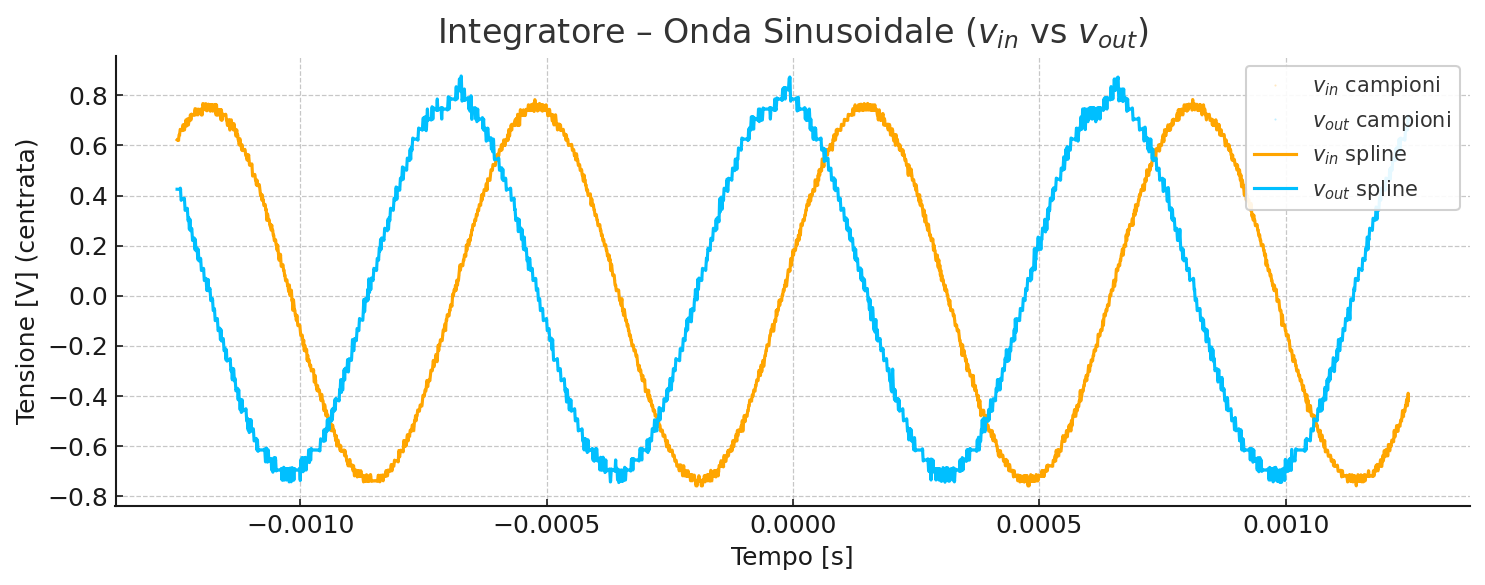
\includegraphics[width=0.9\textwidth]{Sinosuidale2.png}
  \caption{Integratore RC – risposta a onda sinusoidale centrata}
  \label{fig:integratore_sin}
\end{figure}

Come mostrato nella figura \ref{fig:integratore_sin}, il segnale in uscita appare come una sinusoide sfasata in avanti di \(\frac{\pi}{2}\), in perfetto accordo con la relazione teorica \eqref{eq: integratore_sin}. È anche evidente la natura invertente del circuito, che introduce un segno negativo nell’uscita. L’ampiezza del segnale in uscita è risultata essere \(V_{pp,out} = (1.570\,\pm\,0.004)\,\mathrm{V}\), portando a un rapporto sperimentale:
\[
\left| \frac{V_{pp, out}}{V_{pp, in}} \right| = \frac{0.785 \pm 0.015}{0.750 \pm 0.015} = 1.047 \pm 0.004
\]

che risulta pienamente compatibile con il valore teorico previsto dalla relazione:
\[
\left| H(f_{in}) \right| = \frac{1}{2\pi f \tau} = (1.03 \pm 0.07)
\]

\vspace{0.3cm}
\textbf{Onda triangolare.}
Successivamente abbiamo alimentato il circuito con un’onda triangolare, mantenendo frequenza e ampiezza invariati.

\begin{figure}[H]
  \centering
  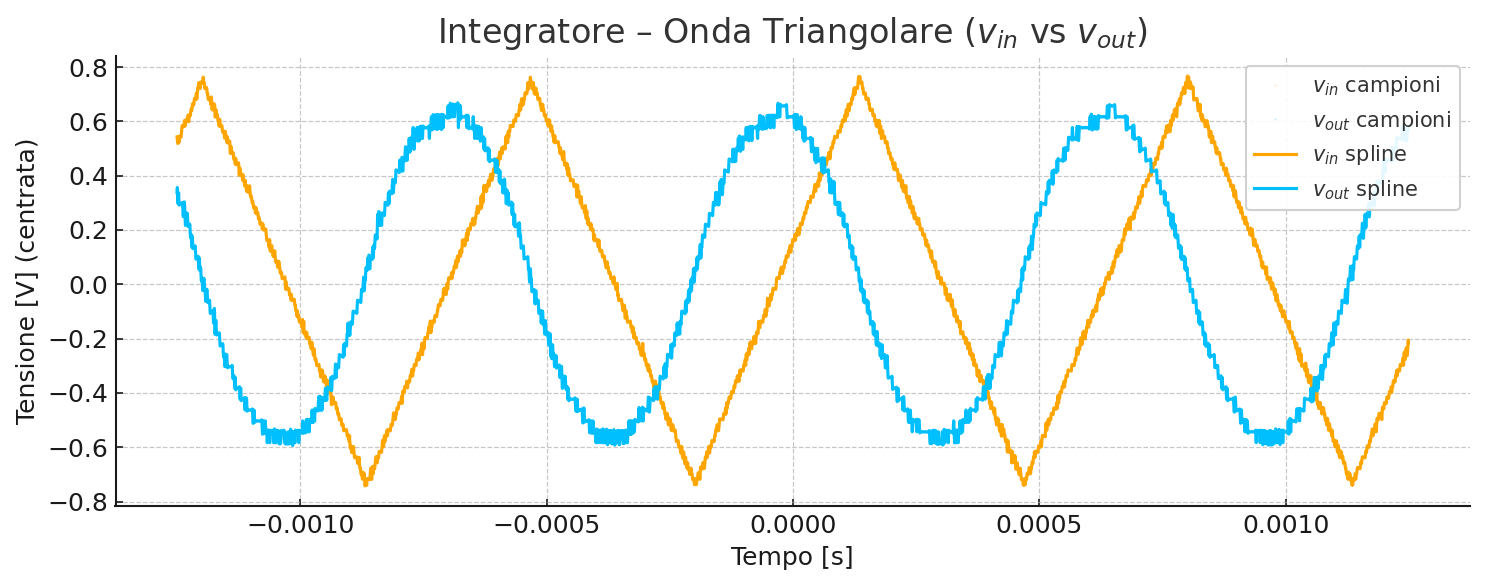
\includegraphics[width=0.9\textwidth]{Triangolare2.png}
  \caption{Integratore RC – risposta a onda triangolare centrata}
  \label{fig:integratore_triang}
\end{figure}

La figura \ref{fig:integratore_triang} mostra una forma d’onda uscente composta da segmenti a parabola, in alternanza tra concavità opposte, come previsto teoricamente per l’integrale di una funzione lineare a tratti. Si osserva che i massimi dell’onda integrata coincidono con i punti in cui l’onda triangolare cambia pendenza. 

L’ampiezza del segnale in uscita è risultata essere \(V_{pp,out} = (1.220\,\pm\,0.004)\,\mathrm{V}\), corrispondente a:
\[
\left| \frac{V_{pp, out}}{V_{pp, in}} \right| = 0.813 \pm 0.003
\]
La cui misura è da confrontare con il valore teorico atteso, la cui formula è stata ottenuta calcolato
integrando il valore di \(v_{in}\), in un tratto lineare, e valutata sul mezzo periodo \(\frac{T}{2}=\frac{1}{2f}\), ottenendo perciò un guadagno di 
\[
\left| H(f_{in}) \right| = \frac{1}{8 f \tau} = 0.810 \pm 0.005
\]
Anche in questo caso, i risultati sperimentali sono compatibili con quelli teorici entro le incertezze.

\vspace{0.3cm}
\textbf{Onda Quadra.}
Infine abbiamo testato il circuito con un’onda quadra di frequenza e ampiezza identiche alle precedenti.

\begin{figure}[H]
  \centering
  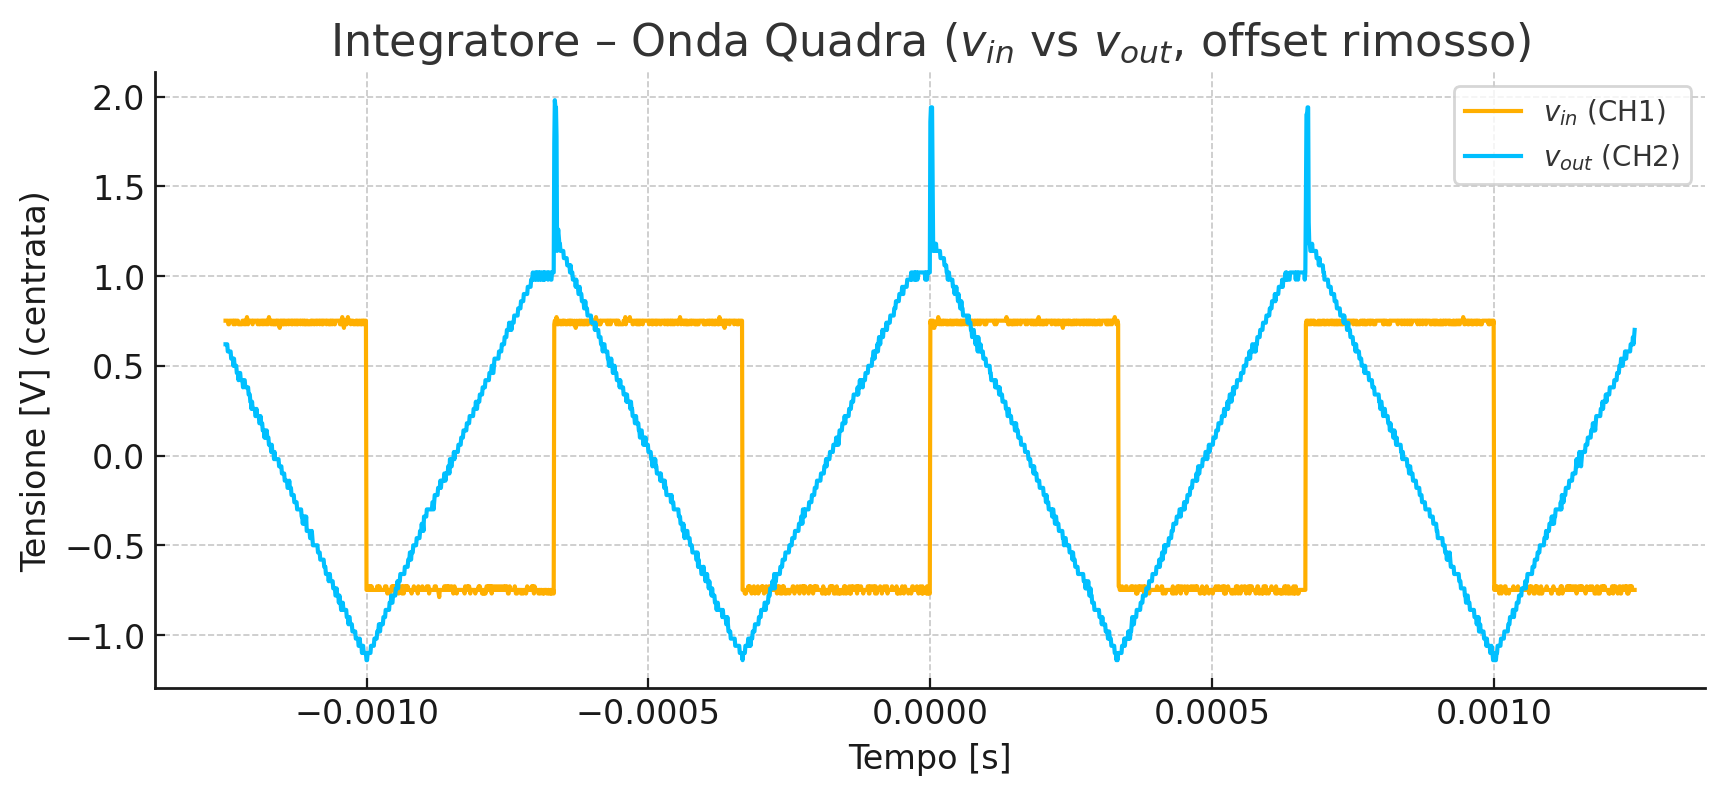
\includegraphics[width=0.9\textwidth]{Quadrata2.png}
  \caption{Integratore RC – risposta a onda quadra centrata}
  \label{fig:integratore_quadra}
\end{figure}

Come mostrato nella figura \ref{fig:integratore_quadra}, il circuito ha risposto come atteso: l’integrale di un’onda quadra è una sequenza di rampe lineari, che in questo caso formano una onda triangolare, invertita rispetto al segnale in ingresso. 
L’andamento lineare delle rampe conferma che il segnale in ingresso resta costante tra due transizioni, e l’inclinazione dipende proporzionalmente dal livello del gradino.

L’ampiezza misurata dell’uscita è stata \(V_{pp,out} = (1.980\,\pm\,0.004)\,\mathrm{V}\) il cui valore era quello mostrato sul display dell'oscilloscopio. Cercando di stimare il guadagno otteniamo
\[
\left| \frac{V_{pp, out}}{V_{pp, in}} \right| = 1.320 \pm 0.004
\]
Il cui valore si discosta da quello atteso, calcolato integrando una costante e valutando la \(v_{out}\) in \(t = \frac{T}{2} =\frac{1}{2f}\), di 
\[
\left| H(f_{in}) \right| = \frac{1}{2 f \tau} = 1.03 \pm 0.02
\]
il che si discosta dal valore teorico atteso di circa 13 deviazioni standard, rendendo le misure incompatibili. Lo scostamento può essere giustificato dalla limitazione della velocità di risposta (slew-rate) e dalla saturazione dinamica del guadagno per frequenze più alte.

Nei punti di transizione dell’onda quadra, l’uscita dell’integratore presenta dei picchi inattesi. Anche in questo caso, tali anomalie sono imputabili a diversi fattori legati alla non idealità dell’amplificatore operazionale. Innanzitutto, la limitata banda passante dell’LM741 impedisce la corretta amplificazione delle componenti ad alta frequenza contenute nei fronti ripidi del segnale, che vengono attenuate, causando una distorsione della risposta impulsiva attesa. Inoltre, il limite di slew-rate (\(\approx 0.5\,\mathrm{V}/\mu\mathrm{s}\)) impedisce all’uscita di variare istantaneamente con la velocità richiesta, generando un sovra/undershoot iniziale. La combinazione di questi fattori produce una risposta transitoria smorzata, amplificata dalla presenza di capacità e induttanze parassite nel circuito.

\section{Analisi dei Circuiti nel Dominio della Frequenza}
Sono stati assemblati un circuito Derivatore RC ed un circuito Integratore CR, come descritti nei paragrafi precedenti. Le componenti utilizzate sono rimaste invariate, elencate nel paragrafo \ref{componenti}.

Per ognuno dei due circuiti sono stati impostati segnali sinusoidali $v_{in}(t)$ in ingresso di diverse frequenze e con un'ampiezza picco-picco selezionata di $V_{pp} = (\,2.000\,\pm 0.004\,) \,\mathrm{V}$, in modo da misurare tramite oscilloscopio ampiezza picco-picco in entrata e in uscita, e calcolare il guadagno in decibel ad ogni freqenza, il che consente di tracciare sperimentalmente il diagramma di Bode che raffigura l'andamento del guadagno in decibel $G(f)$ al variare della freqeunza.

Si è inoltre tracciato il diagramma di Bode che esprime l'andamento dello sfasamento $\phi(f)$, della sinusoide del segnale in uscita rispetto alla sinusoide in entrata, in funzione della frequenza. Lo sfasamento è calcolabile tramite la formula $\phi = 2\pi\frac{\Delta t}{T} = 2\pi\Delta tf $, dove $\Delta t$ è la distanza temporale tra due zeri successivi della sinusoide in ingresso e quella in uscita, misurabile tramite gli appositi cursori di cui l'oscilloscopio è fornito. Tale intervallo temporale è da considerare con segno positivo nel caso in cui la sinusoide in uscita anticipi quella in entrata e con segno negativo in caso di ritardo, in modo da ottenere il segno corretto dello sfasamento.

I diagrammi di Bode ricavati sperimentalmente sono stati confrontati con quelli ottenibili mediante simulazione eseguita con LTSpice.
\subsection{Circuito Derivatore RC}
Di seguito sono riporati e commentati i diagrammi di Bode ottenuti mediante simulazione e sperimentalmente. In fase di esperimento sono stati ottenuti dati in corrispondenza di frequenze in un range di $[0.25, 5000] \,\mathrm{kHz}$. Gli intervalli temporali sono stati presi con segno negativo.

\begin{figure}[H]
  \centering
  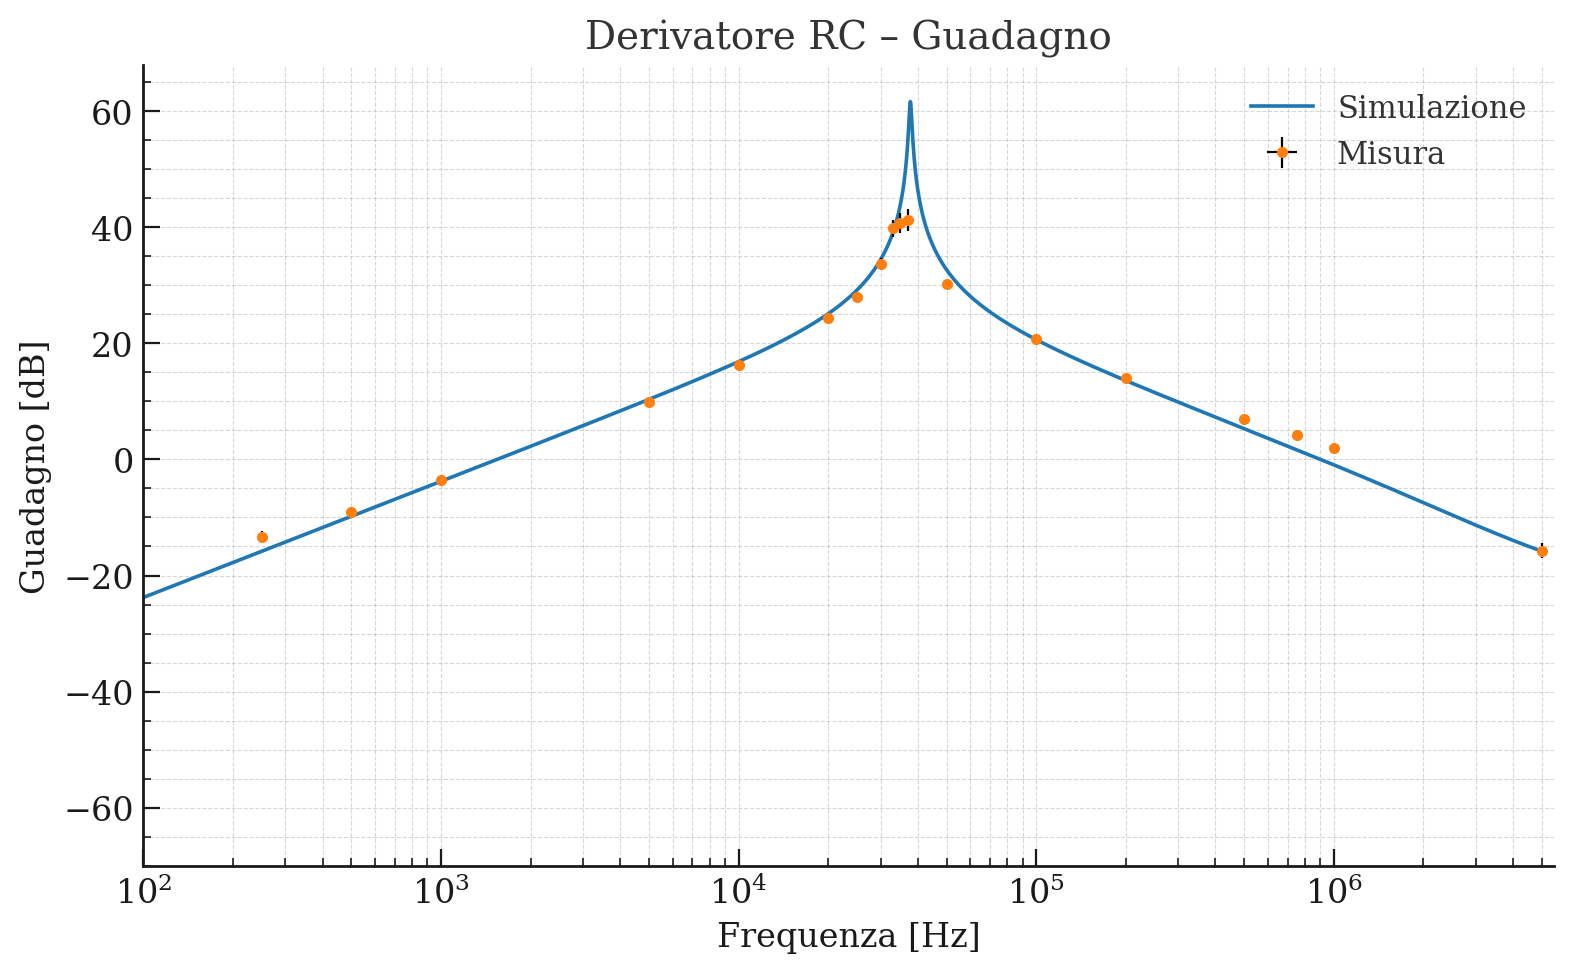
\includegraphics[width=.8\textwidth]{Derivatore_guadagno.png}
  \caption{Diagramma di Bode del guadagno $G(f)$ per il circuito Derivatore RC, confronto tra simulazione e dati sperimentali.}
\end{figure}

\begin{figure}[H]
  \centering
  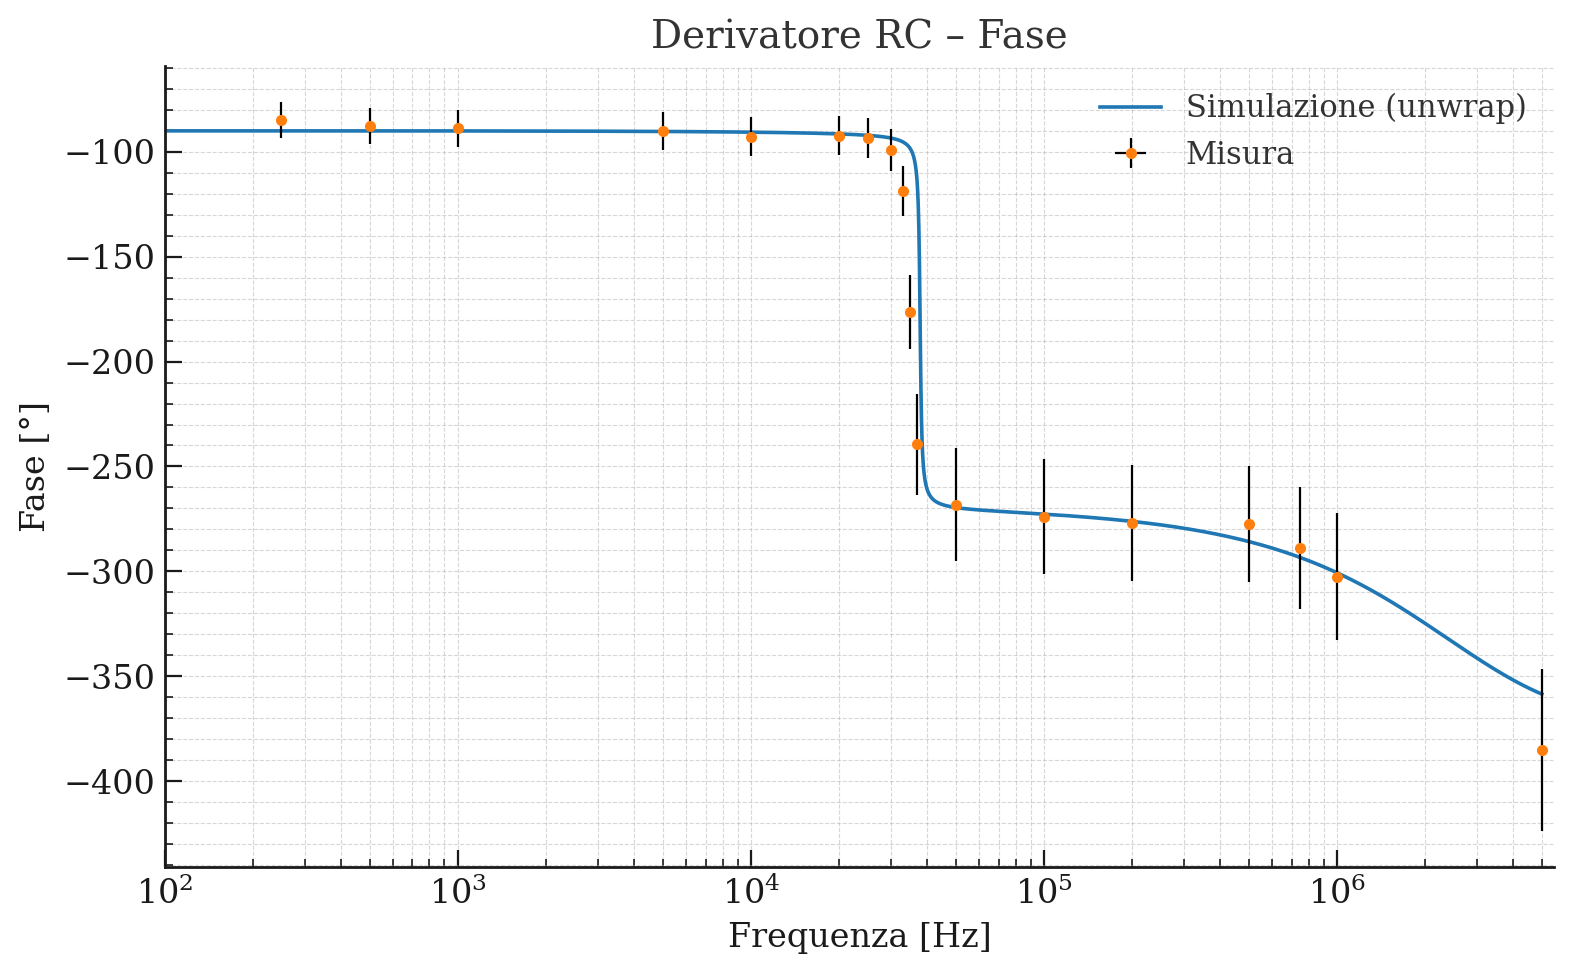
\includegraphics[width=.8\textwidth]{Derivatore_fase.png}
  \caption{Diagramma di Bode dello sfasamento $\phi(f)$ per il circuito Derivatore RC, confronto tra simulazione e dati sperimentali.}
\end{figure}

Si noti come, sia nei dati di simulazione che in quelli ottenuti sperimentalmente, nel range di frequenze comprese tra l’Hz e i \(\SI{300}{\kilo\hertz}\), l’andamento del guadagno è lineare in scala logaritmica, con una pendenza sperimentale pari a \(m = (+19.6 \pm 0.8)\,\frac{dB}{decade}\), ottenuta mediante regressione lineare pesata sui dati a bassa frequenza. Questo valore è in ottimo accordo con la pendenza teorica attesa per un circuito derivatore ideale, pari a \(+20\,\si{\frac{SI{\decibel}}{decade}}\). Anche la fase, per tutto questo intervallo, resta prossima al valore atteso di \(-\frac{\pi}{2}\), coerente con quanto previsto dalla relazione \ref{eq:guadagno_der}.

Alla frequenza \(f_{\mathrm{max}} = (37 \pm 2)\,\si{\kilo\hertz}\), si osserva un picco nel guadagno, con valore massimo \(G_{\mathrm{max}} = (41.3 \pm 1.9)\,\si{\decibel}\) \footnote{Entrambe le incertezze sulla \(f_{max}\) e  \(G_{max}\) sono state valutate con semidispersione massima}, accompagnato da un rapido cambiamento di fase, che nell’oscilloscopio si manifesta come una inversione del segnale. La simulazione riporta un valore di picco leggermente superiore, pari a \(G_{\mathrm{max,sim}} = 61.6\,\si{\decibel}\), localizzato in \(f_{\mathrm{max,sim}} = 37.76\,\si{\kilo\hertz}\).

% Questo fenomeno è causato da un effetto di risonanza, dovuto alla combinazione della rete RC con le capacità parassite del circuito e il comportamento in frequenza dell’amplificatore operazionale. Tali effetti di risonanza emergono quando nel denominatore della funzione di trasferimento compaiono poli complessi coniugati, la cui parte reale si annulla e la parte immaginaria si annulla, amplificando il modulo della risposta in frequenza.
Questo fenomeno è causato dalla risposta in frequenza non ideale dell’amplificatore operazionale, che introduce un comportamento dinamico assimilabile a un singolo polo dominante \( A(s) = A_0/(1 + s/\omega_a) \).\footnote{%
\( A_0 \) è il guadagno a bassa frequenza (tipicamente \( \sim 10^5 \) per LM741) e \( \omega_a \) è la pulsazione di taglio del polo dominante dell’amplificatore, indicativamente pari a \( \sim 2\pi \cdot 5\,\si{\radian\per\second} \).%
}
Quando il circuito derivatore viene chiuso in retroazione negativa, questa dinamica si riflette nella funzione di trasferimento complessiva, che assume la forma:

\[
H(s) = -\frac{\tau A_0}{\omega_a} \cdot \frac{s}{s^2 + 2\zeta\omega_n s + \omega_n^2}
\]

dove \( \omega_n = \sqrt{A_0 \omega_a / \tau} \)\footnote{%
\( \omega_n \) è la pulsazione naturale del sistema risonante equivalente, determinata dalla combinazione tra la dinamica dell'amplificatore e la costante di tempo del circuito RC.%
}
è la pulsazione naturale del sistema e \( \zeta = (1 + A_0)/(2\sqrt{A_0}) \)\footnote{%
\( \zeta \) è il coefficiente di smorzamento: rappresenta il rapporto tra le componenti dissipative e reattive del sistema, ed è responsabile della presenza (o assenza) di un picco di risonanza.%
}
è il coefficiente di smorzamento. In queste condizioni compaiono nel denominatore due poli complessi coniugati, la cui presenza è responsabile del comportamento risonante del modulo. Quando lo smorzamento è basso (\( \zeta < 1/\sqrt{2} \)), il circuito presenta un picco di guadagno in corrispondenza della frequenza

\[
f_{\text{peak}} = \frac{\omega_n}{2\pi} \sqrt{1 - 2\zeta^2}
\]

corrispondente a quanto osservato sperimentalmente. Il modulo della risposta si amplifica in prossimità di tale frequenza, spiegando matematicamente il comportamento osservato nei dati.

Nel nostro caso, le misure hanno mostrato un picco di guadagno pari a \( G_{\text{max}} = (\,41.3\, \pm\, 1.9\,)\,\si{\decibel} \) in corrispondenza della frequenza \( f_{\text{peak}} = (\,37\, \pm\, 2\,)\,\si{\kilo\hertz} \), mentre la simulazione LTspice ha previsto un valore massimo di \( G_{\text{max,sim}} = 61.6\,\si{\decibel} \) a \( f_{\text{peak,sim}} = 37.76\,\si{\kilo\hertz} \). La discrepanza in ampiezza è attribuibile al limitato slew-rate dell’LM741, mentre l’ottimo accordo sulla posizione del picco conferma la validità del modello analitico.

Il guadagno unitario è stato raggiunto in due distinte frequenze:
\[
f_{0,1} = (1.486 \pm 0.073)\,\si{\kilo\hertz}, \quad
f_{0,2} = (1.044 \pm 0.071)\,\si{\mega\hertz}
\]
rispettivamente nelle zone di salita e discesa del guadagno. La prima coincide con la frequenza caratteristica calcolata teoricamente tramite l’equazione \eqref{eq: freqenza_carr}, mentre la seconda appare come effetto della compensazione interna dell’amplificatore.

Da notare come, superato il \si{\mega\hertz}, il segnale si attenua significativamente e la fase diminuisce drasticamente fino a tornare a una fase di \(-2\pi\), annullandosi. Questo comportamento è imputabile alla presenza di una capacità di giunzione interna all’LM741, approssimabile a un condensatore posto in parallelo all’ingresso dell’amplificatore. A frequenze elevate, questa capacità diventa dominante, facendo sì che il segnale bypassi l’amplificatore, che presenta un tempo di risposta finito. Di conseguenza, il segnale in uscita risulta fortemente attenuato e in fase con l’ingresso, vanificando l’effetto derivativo previsto dal modello ideale.

% \subsection{Circuito Integratore RC}
% Per quanto riguarda il circuito Integratore RC. In fase di esperimento sono stati ottenuti dati in corrispondenza di frequenze in un range di $[0.015, 5000s] \,\mathrm{kHz}$. Gli intervalli temporali sono stati presi con segno positivo.

% Di seguito sono riportati gli output delle simulazioni e le misurazioni e i diagrammi di Bode ricavati sperimentalmente.

% \begin{figure}[htbp]
%   \centering
%   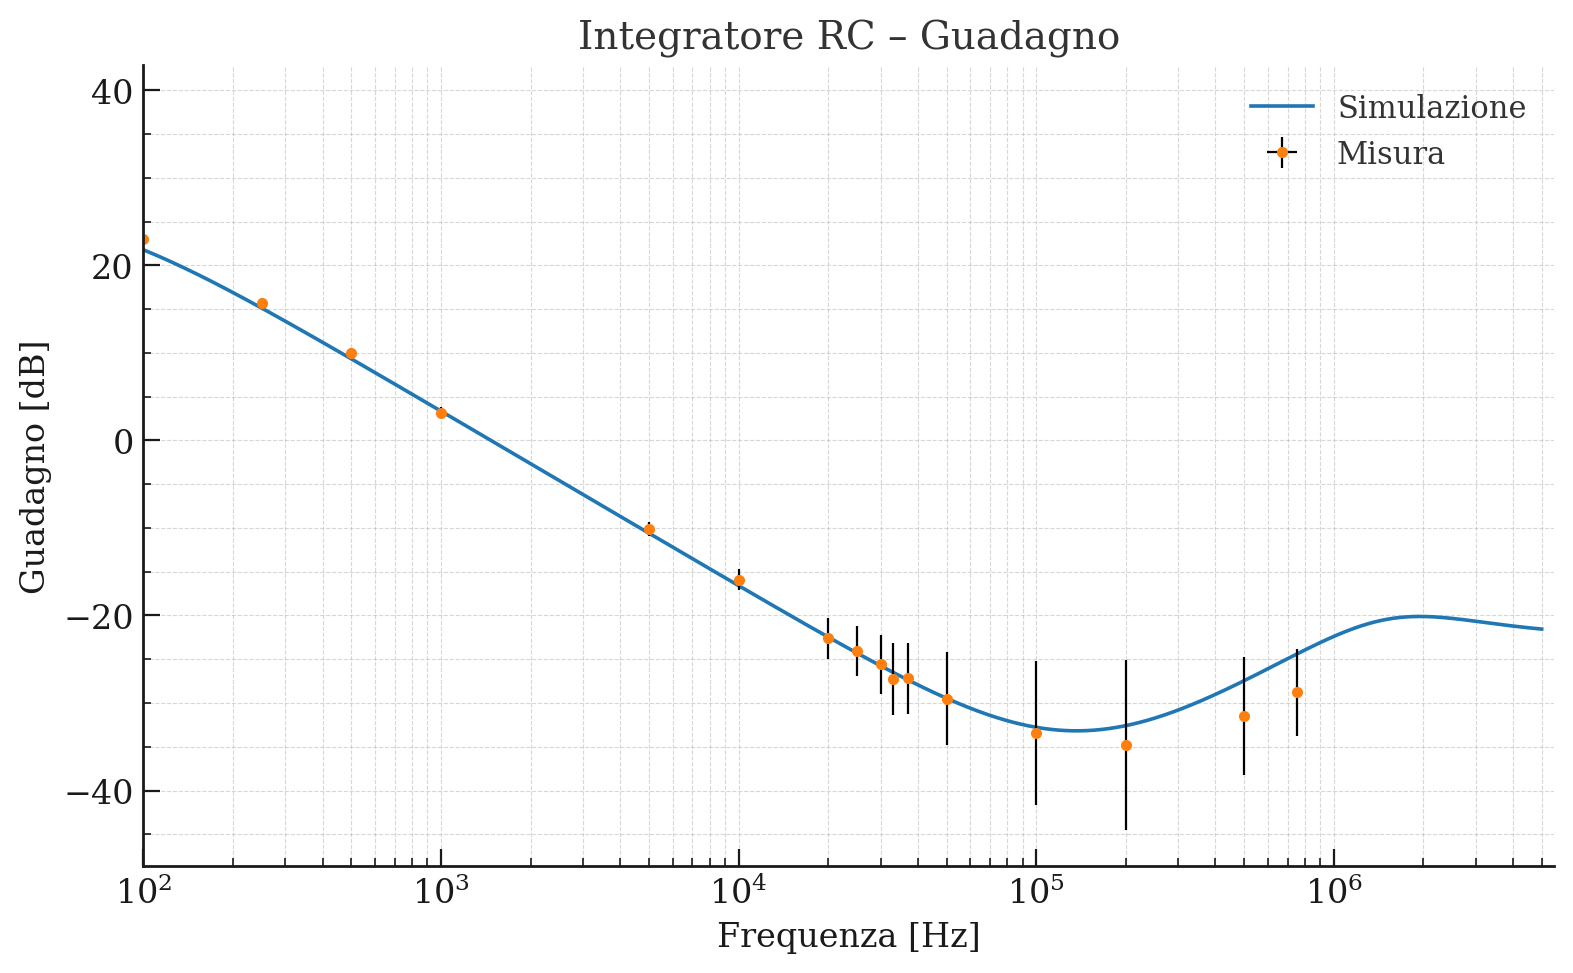
\includegraphics[width=.8\textwidth]{Integratore_guadagno.png}
%   \caption{Diagrammi di Bode di G(f), circuito Integratore RC}
% \end{figure}

% \begin{figure}[htbp]
%   \centering
%   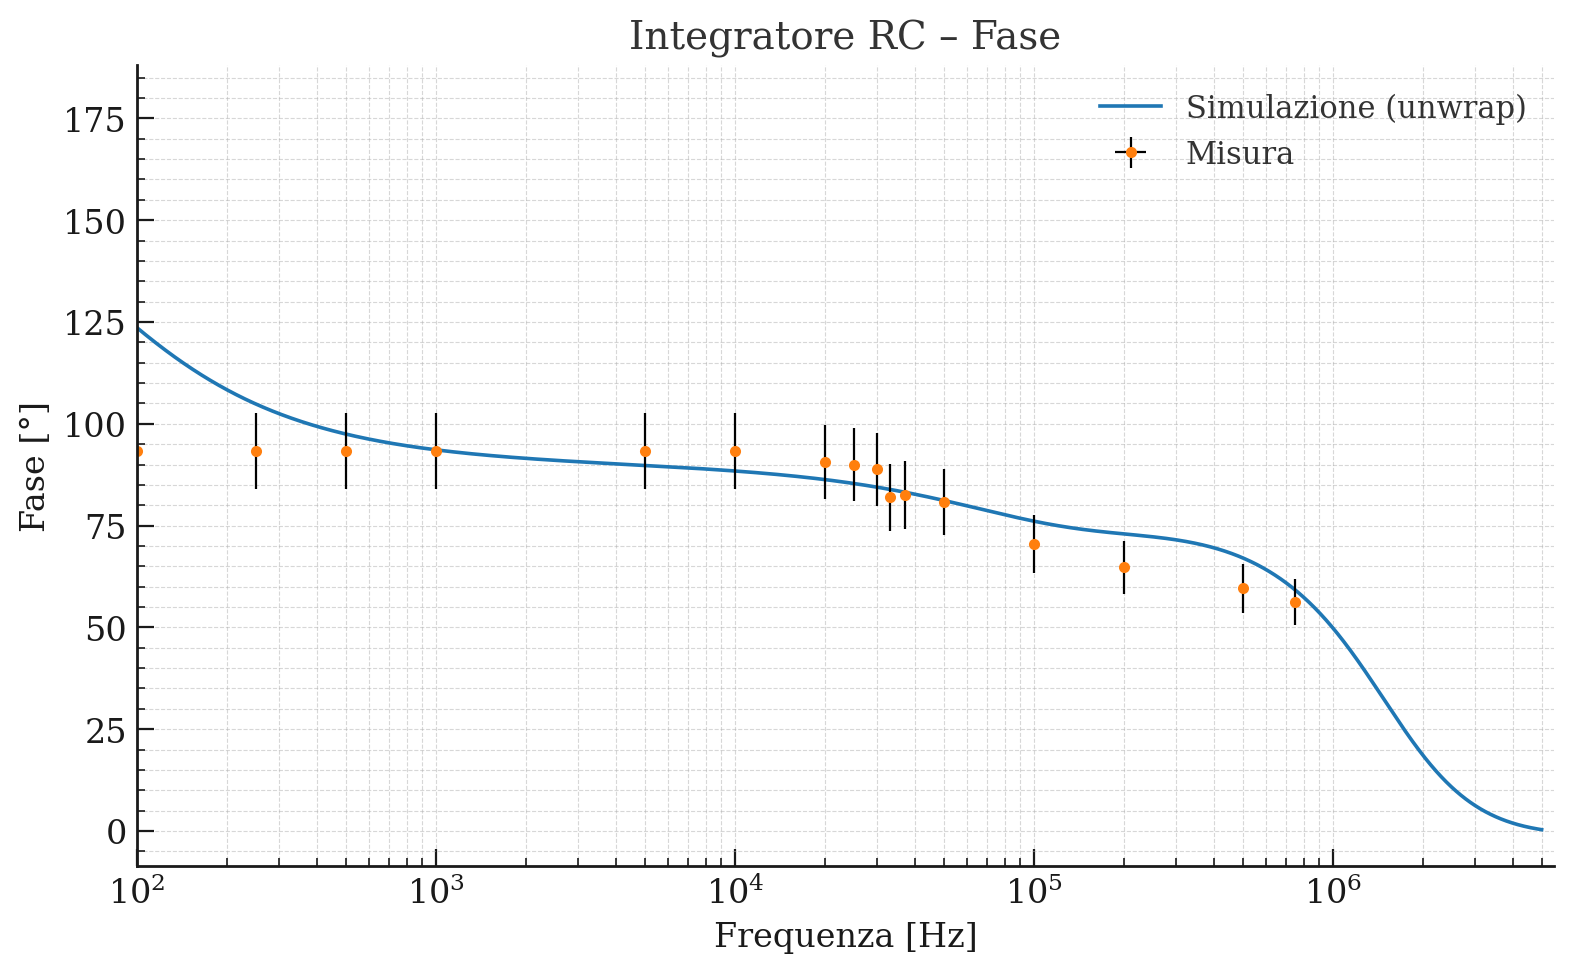
\includegraphics[width=.8\textwidth]{Integratore_fase.png}
%   \caption{Simulazioni Diagrammi di Bode di  $\phi(f)$, circuito Derivatore RC}
% \end{figure}

% Come si nota, è possibile fare considrazioni analoghe a quelle riguardanti il circuito Derivatore. 
% Come è atteso secondo la relazione \ref{10} il modulo della Risposta in frequenza risulta inversamnte proporzionale alla frequenza, perciò per la relazione \ref{eq: Gdb} otteniamo un andamento lineare negativo del Guadagno all'interno di un intervallo di frequenze che va da quelle da cui abbiamo iniziato a misurare fino a circa i 100kHz.
% Sia nei dati sperimentali che nel risultato delle simulazioni abbiamo ottenuto dei valori minimi di guadagno. Se ne confrontiamo i valori:
% fmin,sim =  , fmin,dati= 2e5pm x
% osserviamo che hanno una compatibilità del ...  Il che conferma una forte corrispondenza tra la simulazione e il circuito sperimentale.
% Le frequenze in questa zona sono molto lontane dalla frequenza caratteristica fc il circuito inizia a comportarsi in maniere imprevedibile. 
% Notiamo però una sostanziale differenza in come si comporta a basse frequenze, in particolare si nota che, mentre nella presa dato abbiamo un comportamento lineare anche su frequenze sotto i 100Hz, nelle simulazioni otteniamo invece dei valori piuttosto costanti. Questo lo possiamo attribuire alle approssimazioni di condensatore ideale sfruttate da LTspice. Questo è sostenuto dal fatto che, mentre un condensatore reale possiede una resistenza in serie che fa passare comunque corrente anche a basse frequenze, un condensatore ideale no, queso non permette alla
% Quando il condensatore nell’integratore risulta carico esso non fornisce più un percorso di retroazione, funziona
% come un circuito aperto, facendo saturare l’uscita dell’Amplificatore Operazionale, cosa che nel caso reale è attenuata dall condensatore reale.
% Inserire il valore di Guadagno unitario
% Passando alla fase invece, notiamo che a frequenze basse la fase risulta essere di 180 gradi, ossia comportandosi come un circuito aperto ma invertito. 
% I valori della fase ottenuti sono compatibili con quelli aspettati di PI a basse frequenze e a  ridosso della nostra fc. Superata la soglia delle fmax, la fase inizia a decresecere linearmnte ad un rate di circa... 
% Il valore della fase nella simulazione è invece, man mano che la frequenza si avvicina a quella caratteristica del circuito \(f_c = ...\) la fase si assesta sul valore atteso di 90 gradi, per poi riprendere a decrescere lentamente fino ad un Mz, dove decresce rapidamente per annullarsi.

% Anche in questo caso si può notare come, superato il MHz il segnale si attenua e la fase diminuisce drasticamente fino a toranare ad una fase di \(-2\pi\), annullandosi. Anche in questo caso  questo caso, il comportamento è  dovuto dalla presenza di una capacità di giunzione dell'amplificatore LM741, approssimabile ad un  condensatore collegato in parallelo all'amplificatore.
% Anche questa discrepanza tra i valori ottenuti e simulati è da attribuire alla approssimazione di condensatore ideale nel software di simulazione.
\subsection{Circuito Integratore RC}
Per quanto riguarda il circuito Integratore RC, in fase di esperimento sono stati ottenuti dati in corrispondenza di frequenze in un range di $[100\,\mathrm{Hz}, 5\,\mathrm{MHz}]$. Gli intervalli temporali sono stati presi con segno positivo.

Di seguito sono riportati gli output delle simulazioni e le misurazioni e i diagrammi di Bode ricavati sperimentalmente.

Come si nota, è possibile fare considerazioni analoghe a quelle riguardanti il circuito derivatore. Come previsto dalla relazione \eqref{eq: Gdb}, il modulo della risposta in frequenza risulta inversamente proporzionale alla frequenza, il che si traduce in un andamento lineare decrescente del guadagno in dB. Questo comportamento è verificato sperimentalmente fino a circa \(f = 100\,\mathrm{kHz}\), dove il circuito segue il modello ideale dell'integratore.

\begin{figure}[H]
  \centering
  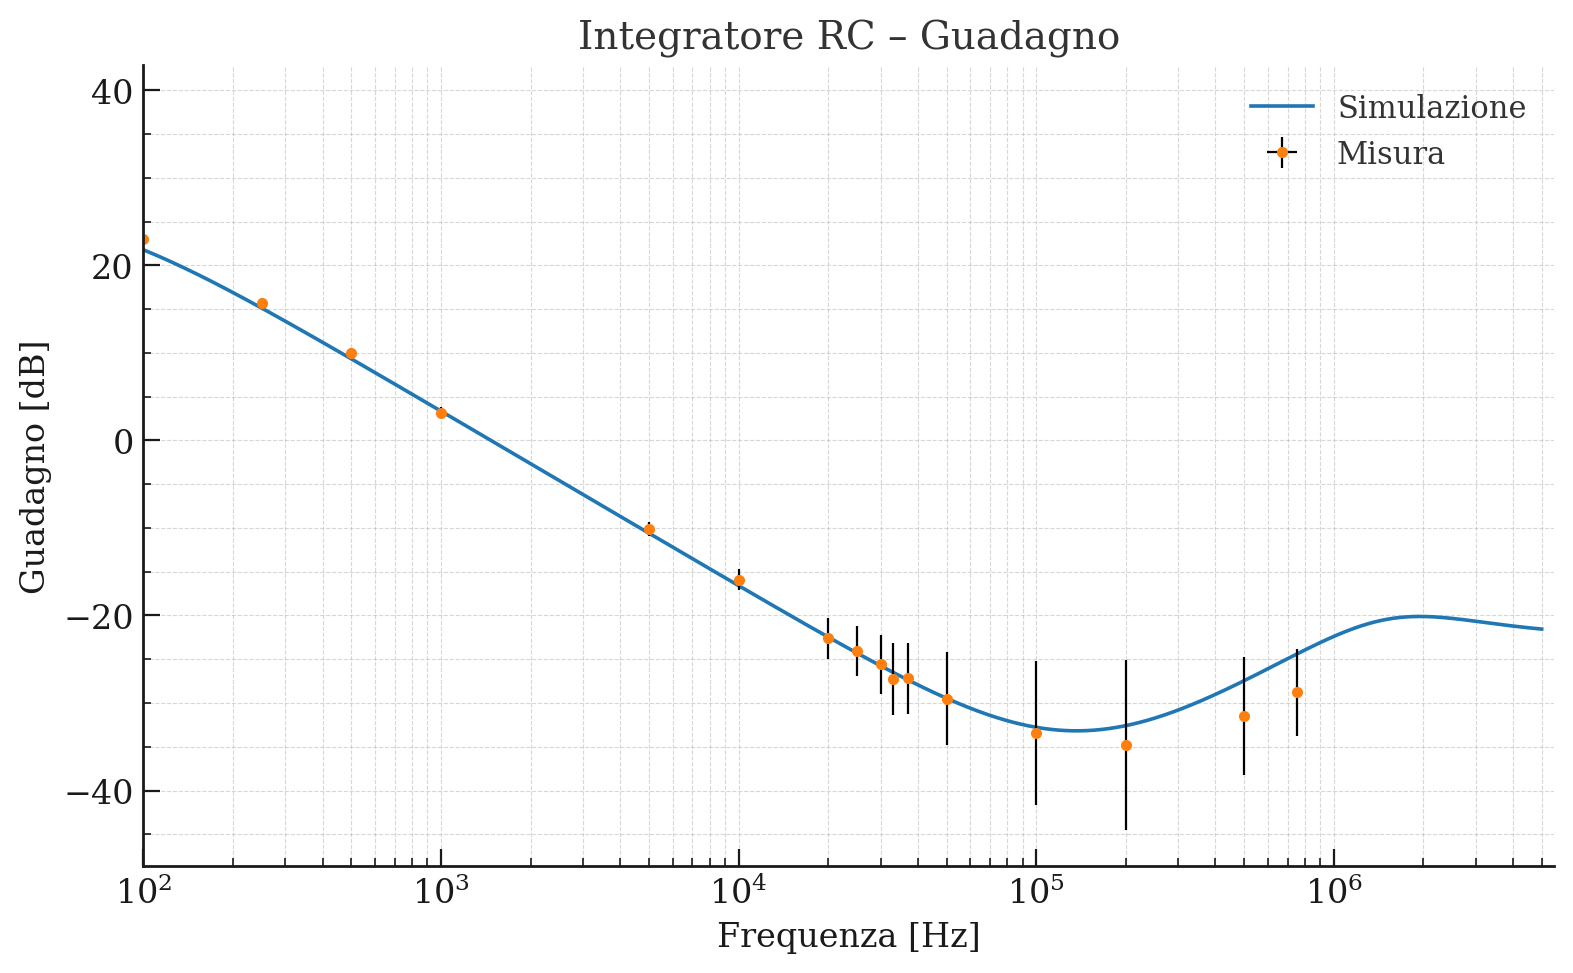
\includegraphics[width=.8\textwidth]{Integratore_guadagno.png}
  \caption{Diagrammi di Bode di $G(f)$, circuito Integratore RC}
\end{figure}

\begin{figure}[H]
  \centering
  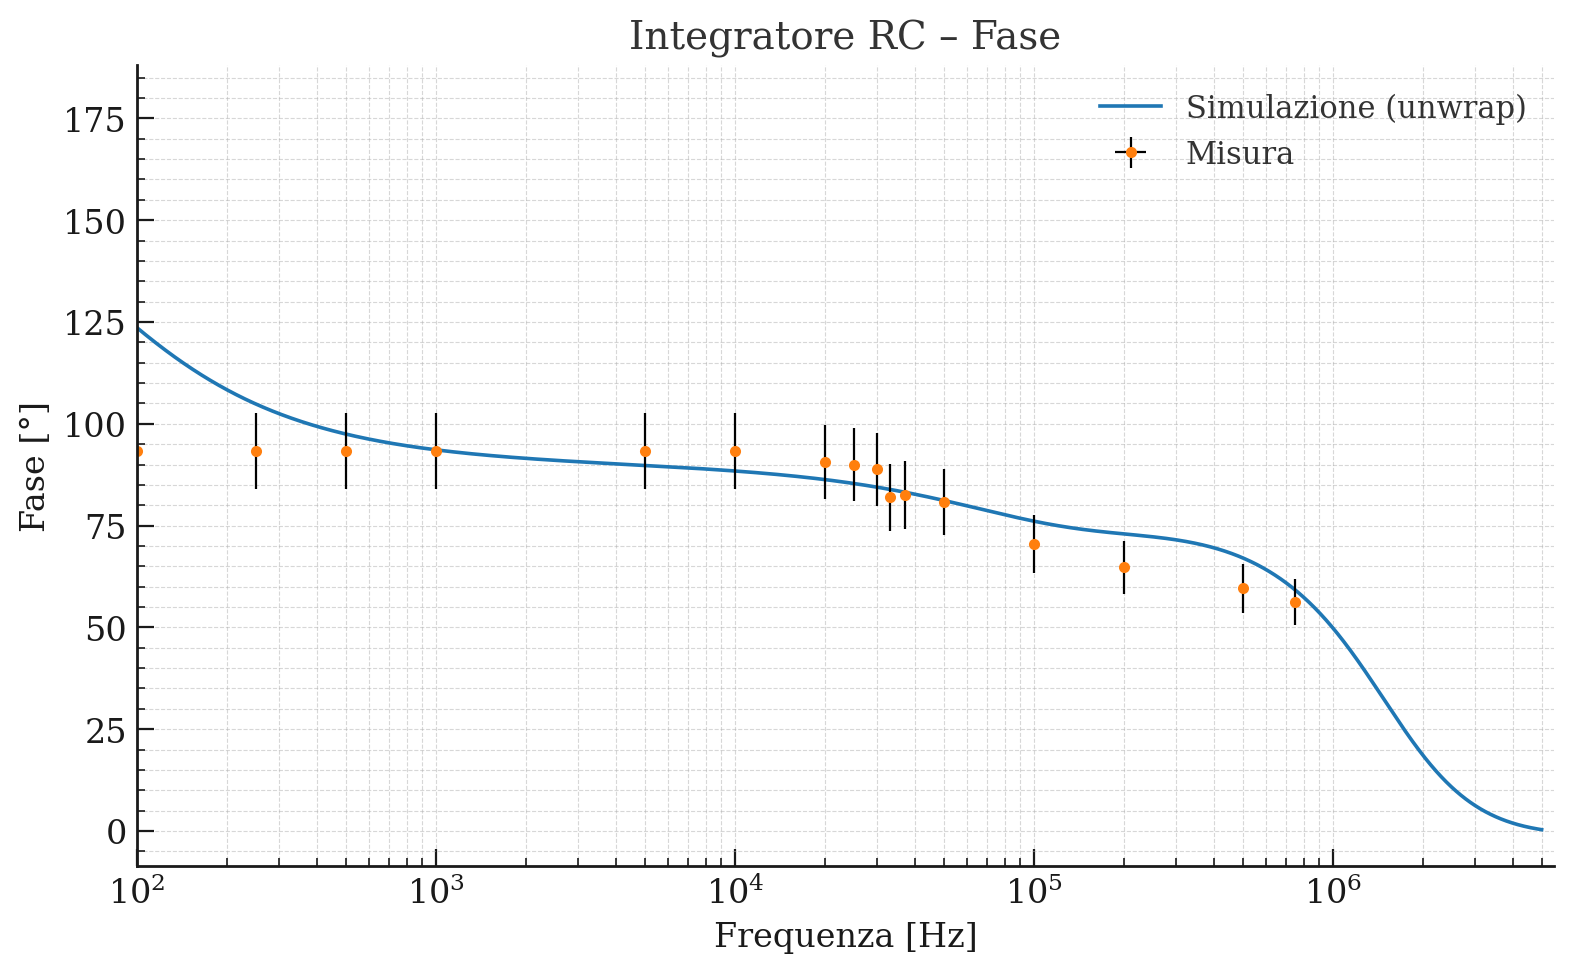
\includegraphics[width=.8\textwidth]{Integratore_fase.png}
  \caption{Diagrammi di Bode di $\phi(f)$, circuito Integratore RC}
\end{figure}

Una regressione lineare pesata sui dati nel range \(15\,\mathrm{Hz} \leq f \leq 5\,\mathrm{kHz}\) ha restituito una pendenza sperimentale del guadagno pari a \(m = (-19.16 \pm 0.32)\,\mathrm{dB/decade}\), in ottimo accordo con il valore teorico atteso di \(-20\,\mathrm{dB/decade}\). L'intercetta dell'interpolazione \(q = (61.17 \pm 0.77)\,\mathrm{dB}\) consente di stimare la frequenza caratteristica sperimentale, ossia di guadagno unitario:
\[
f_c = (1.56 \pm 0.07)\,\mathrm{kHz}
\]
in eccellente compatibilità con il valore teorico \(f_{c,\mathrm{teo}} = (1.546 \pm 0.001)\,\mathrm{kHz}\) calcolato a partire dai valori di \(R\) e \(C\) misurati.

Si osserva anche un valore minimo del guadagno pari a \(G_{\min} = (-34.8 \pm 1.0)\,\mathrm{dB}\) in corrispondenza di \(f_{\min} = (200 \pm 10)\,\mathrm{kHz}\), ben riprodotto dalla simulazione. Ciò conferma una buona corrispondenza tra il circuito reale e il modello simulato, anche oltre la regione di validità del comportamento ideale.

Le frequenze in questa zona sono molto lontane dalla frequenza caratteristica \(f_c\) e il circuito inizia a comportarsi in maniera non ideale. A frequenze ancora più elevate (\(f > 500\,\mathrm{kHz}\)) si osserva un'inversione di tendenza del guadagno, che ricomincia ad aumentare: tale fenomeno è riconducibile alla limitata banda passante dell'amplificatore LM741 e alla presenza di capacità parassite.

Un'altra discrepanza interessante si osserva alle basse frequenze: mentre i dati sperimentali mostrano un andamento lineare del guadagno anche sotto i \(100\,\mathrm{Hz}\), la simulazione tende a produrre un guadagno costante in tale regione. Questo può essere attribuito all'approssimazione del condensatore come elemento ideale in LTspice. I condensatori fisici presentano una resistenza serie equivalente, che consente il passaggio di corrente anche a bassa frequenza. Quando il condensatore risulta completamente carico, in un modello ideale non fornisce più alcun percorso di retroazione, comportandosi come un circuito aperto e portando l’amplificatore in saturazione. Nel circuito reale, l’effetto è mitigato proprio da questa resistenza e da eventuali resistenze parassite o intenzionalmente inserite in parallelo al condensatore.

Passando all’analisi della fase, si osserva che a frequenze basse la fase si attesta a circa \(180^\circ\), coerentemente con il comportamento di un circuito invertente in condizioni di circuito aperto. Nell'intervallo in cui il circuito si comporta come un integratore ideale (\(f < 100\,\mathrm{kHz}\)), la fase si mantiene prossima al valore atteso di \(\varphi = (+90)^\circ\). All’aumentare della frequenza, la fase comincia a decrescere lentamente fino a circa \(f = 1\,\mathrm{MHz}\), oltre il quale cala rapidamente, fino ad annullarsi.

Anche in questo caso si può notare come, superato il \si{\mega\hertz}, il segnale si attenua e la fase diminuisce drasticamente fino a tornare a \(-2\pi\), ovvero a fase nulla. Questo comportamento è dovuto alla capacità di giunzione dell’amplificatore LM741, che si comporta come un condensatore collegato in parallelo all’amplificatore e che diventa dominante alle alte frequenze. Tale comportamento impedisce la corretta retroazione e rende inefficace l’azione integrativa. 

\end{document}